% Hermes AI 연구실 설치 매뉴얼 — INSTALL.md를 처음 하는 사람용으로 풀어 쓴 LaTeX판
% 빌드: xelatex INSTALL.tex  (두 번 돌리면 목차와 쪽 번호가 채워진다)
% 필요: texlive-xetex, texlive-lang-korean(kotex), texlive-latex-extra(fvextra, tcolorbox), texlive-pictures(tikz)
% 글꼴: Noto Sans CJK KR, D2Coding ligature
\documentclass[10pt,a4paper,oneside]{report}

\usepackage[top=24mm,bottom=24mm,left=22mm,right=22mm,headheight=14pt]{geometry}
\usepackage{kotex}
\setmainfont{Noto Sans CJK KR}[UprightFont={* DemiLight},BoldFont={* Bold}]
\setsansfont{Noto Sans CJK KR}[UprightFont={* DemiLight},BoldFont={* Bold}]
\setmonofont{D2Coding ligature}[Scale=0.92,HyphenChar=None,Ligatures={NoCommon,NoContextual,NoRequired},RawFeature={-calt}]
\setmainhangulfont{Noto Sans CJK KR}[UprightFont={* DemiLight},BoldFont={* Bold}]
\setsanshangulfont{Noto Sans CJK KR}[UprightFont={* DemiLight},BoldFont={* Bold}]
\setmonohangulfont{D2Coding ligature}[Scale=0.92,HyphenChar=None,Ligatures={NoCommon,NoContextual,NoRequired},RawFeature={-calt}]

\usepackage[table]{xcolor}
\usepackage{array,booktabs,longtable,tabularx}
\usepackage{enumitem}
\usepackage{fvextra}
\usepackage[most]{tcolorbox}
\usepackage{tikz}
\usepackage{graphicx}
\usetikzlibrary{positioning,fit,arrows.meta,backgrounds,calc}
\usepackage{titlesec}
\usepackage{fancyhdr}
\usepackage{tocloft}
\usepackage{amssymb}
\usepackage[hidelinks]{hyperref}

% ---------------------------------------------------------------- 색
\definecolor{accent}{HTML}{0E7C86}      % 제목·강조 (청록)
\definecolor{navy}{HTML}{1B2A47}        % 표지·장 제목 띠
\definecolor{accentlight}{HTML}{E6F3F4}
\definecolor{ink}{HTML}{1F2328}
\definecolor{muted}{HTML}{6B7280}
\definecolor{codebg}{HTML}{1A2236}      % 명령 상자 (짙은 남색)
\definecolor{codefg}{HTML}{E6E6EF}
\definecolor{inlinefg}{HTML}{24292F}
\definecolor{filebg}{HTML}{FAFAFB}
\definecolor{fileframe}{HTML}{C9CDD3}
\definecolor{outbg}{HTML}{F1F3F5}
\definecolor{tipc}{HTML}{2E9E5B}   \definecolor{tipbg}{HTML}{EEF7F1}
\definecolor{warnc}{HTML}{CC3B3B}  \definecolor{warnbg}{HTML}{FCEFEF}
\definecolor{infoc}{HTML}{2F6FD0}  \definecolor{infobg}{HTML}{EEF3FB}
\definecolor{msgbg}{HTML}{EEF0FE}
\definecolor{discord}{HTML}{5865F2}
\definecolor{okc}{HTML}{2E9E5B}

\color{ink}

% ---------------------------------------------------------------- 쪽 모양
\setlength{\parindent}{0pt}
\setlength{\parskip}{0.55em}
\setlength{\emergencystretch}{3em}
\linespread{1.18}
\setlist{itemsep=0.25em,topsep=0.3em}
\renewcommand{\arraystretch}{1.3}
\setcounter{secnumdepth}{2}
\setcounter{tocdepth}{2}

% 장 제목: 남색 띠 안에 번호와 제목
\newcommand{\chapterbanner}[2]{%
  \begin{tcolorbox}[enhanced,colback=navy,colframe=navy,boxrule=0pt,arc=6pt,
    left=16pt,right=16pt,top=14pt,bottom=14pt,
    borderline south={3pt}{0pt}{accent},before skip=0pt,after skip=0pt]
  #1{\color{white}\fontsize{24}{32}\selectfont\bfseries #2}
  \end{tcolorbox}}
\newcommand{\chaplabel}{{\color{accent!45!white}\small\bfseries CHAPTER \thechapter}\par\vspace{3pt}}
\titleformat{\chapter}[block]{\normalfont}{}{0pt}{\chapterbanner{\chaplabel}}
\titleformat{name=\chapter,numberless}[block]{\normalfont}{}{0pt}{\chapterbanner{}}
\titlespacing*{\chapter}{0pt}{0pt}{20pt}
% 절 제목: 청록 번호 딱지
\newcommand{\secnum}[1]{\tcbox[on line,colback=accent,colframe=accent,boxrule=0pt,arc=3pt,
  left=4pt,right=4pt,top=1pt,bottom=1pt]{\color{white}\large\bfseries #1}}
\titleformat{\section}{\Large\bfseries}{\secnum{\thesection}}{0.6em}{}
\titleformat{\subsection}{\large\bfseries}{\color{accent}\thesubsection}{0.7em}{}
\titleformat{\subsubsection}{\normalsize\bfseries}{}{0em}{}
\titlespacing*{\section}{0pt}{1.6em}{0.6em}
\titlespacing*{\subsection}{0pt}{1.3em}{0.4em}

\renewcommand{\cftchapfont}{\bfseries\color{navy}}
\renewcommand{\cftchappagefont}{\bfseries\color{accent}}
\renewcommand{\cftchappresnum}{\color{accent}}
\setlength{\cftbeforechapskip}{0.9em}
\renewcommand{\cftsecleader}{\cftdotfill{\cftdotsep}}
\renewcommand{\contentsname}{차례}

\pagestyle{fancy}
\fancyhf{}
\renewcommand{\headrulewidth}{0pt}
\renewcommand{\chaptermark}[1]{\markboth{\ifnum\value{chapter}>0 \thechapter.\ \fi#1}{}}
\fancyhead[L]{\small{\color{accent}\rule[-1.5pt]{3pt}{9pt}}\hspace{6pt}{\color{muted}\leftmark}}
\fancyhead[R]{\small\color{muted}Hermes AI 연구실 · 설치 매뉴얼}
\newcommand{\pagepill}{\tcbox[on line,colback=accentlight,colframe=accentlight,boxrule=0pt,arc=6pt,
  left=6pt,right=6pt,top=1pt,bottom=1pt]{\small\bfseries\color{accent}\thepage}}
\fancyfoot[C]{\pagepill}
\fancypagestyle{plain}{\fancyhf{}\fancyfoot[C]{\pagepill}}

% ---------------------------------------------------------------- 상자
% 명령 상자 (검정): 터미널에 그대로 입력하는 명령. 긴 줄은 자동으로 접는다
\DefineVerbatimEnvironment{sh}{Verbatim}{breaklines,breakanywhere,breaksymbolleft={},breakanywheresymbolpre={},
  breakindent=1.5em,fontsize=\small,formatcom=\color{codefg}}
\newtcolorbox{shbox}{enhanced,colback=codebg,colframe=codebg,boxrule=0pt,arc=4pt,
  left=10pt,right=10pt,top=6pt,bottom=6pt,before skip=0.6em,after skip=0.8em}
\BeforeBeginEnvironment{sh}{\begin{shbox}}
\AfterEndEnvironment{sh}{\end{shbox}}

% 파일 상자 (흰색 + 제목): 파일에 적는 내용
\DefineVerbatimEnvironment{code}{Verbatim}{breaklines,breakanywhere,breaksymbolleft={},breakanywheresymbolpre={},breakindent=1.5em,fontsize=\small}
\newtcolorbox{filebox}[1]{enhanced,colback=filebg,colframe=fileframe,boxrule=0.5pt,arc=4pt,
  colbacktitle=outbg,coltitle=ink,fonttitle=\small\ttfamily,title={#1},
  left=8pt,right=8pt,top=4pt,bottom=4pt,before skip=0.6em,after skip=0.8em}

% 출력 상자 (회색): 화면에 나오는 결과 예시
\DefineVerbatimEnvironment{out}{Verbatim}{breaklines,breakanywhere,breaksymbolleft={},breakanywheresymbolpre={},fontsize=\small,formatcom=\color{muted}}
\newtcolorbox{outbox}{enhanced,colback=outbg,colframe=fileframe,boxrule=0.4pt,arc=4pt,
  left=8pt,right=8pt,top=3pt,bottom=3pt,before skip=0.5em,after skip=0.8em}
\BeforeBeginEnvironment{out}{\begin{outbox}}
\AfterEndEnvironment{out}{\end{outbox}}

% Discord에서 보내는 말 (Discord 보라)
\newtcolorbox{msg}[1][Discord에서 보낼 메시지]{enhanced,colback=msgbg,frame hidden,boxrule=0pt,arc=3pt,
  borderline west={3pt}{0pt}{discord},left=10pt,right=8pt,top=5pt,bottom=5pt,
  fontupper=\normalsize,before upper={{\color{discord}\bfseries #1}\par\smallskip},before skip=0.6em,after skip=0.8em}

% 왼쪽 줄 상자: 팁 / 주의 / 정보 / 확인
\newcommand{\sidebox}[4]{%
  \begin{tcolorbox}[enhanced,colback=#2,frame hidden,boxrule=0pt,arc=3pt,
    borderline west={3pt}{0pt}{#1},left=10pt,right=8pt,top=5pt,bottom=5pt,before skip=0.6em,after skip=0.8em]
  {\color{#1}\bfseries #3}\hspace{0.7em}#4
  \end{tcolorbox}}
\newcommand{\tip}[2]{\sidebox{tipc}{tipbg}{#1}{#2}}
\newcommand{\warn}[2]{\sidebox{warnc}{warnbg}{#1}{#2}}
\newcommand{\info}[2]{\sidebox{infoc}{infobg}{#1}{#2}}
\newcommand{\ok}[1]{\sidebox{okc}{white}{\checkmark\ 성공하면}{#1}}

% 인라인 코드, 키, 채널
\newcommand{\cmd}[1]{\textcolor{inlinefg}{\texttt{\detokenize{#1}}}}
\newcommand{\kbd}[1]{\tcbox[on line,colback=white,colframe=fileframe,boxrule=0.4pt,arc=2pt,
  left=2pt,right=2pt,top=0.5pt,bottom=0.5pt,boxsep=0.5pt]{\footnotesize\ttfamily #1}}
\newcommand{\ch}[1]{\texttt{\#}\texttt{#1}}
\newcommand{\does}[1]{\begin{tcolorbox}[enhanced,colback=accentlight,frame hidden,boxrule=0pt,arc=4pt,
  left=8pt,right=8pt,top=4pt,bottom=4pt,before skip=0.2em,after skip=0.6em]
  {\color{accent}\bfseries 이 단계에서 하는 일}\hspace{0.7em}#1\end{tcolorbox}}
\newcommand{\head}{\rowcolor{outbg}}

% 표: 줄바꿈 되는 왼쪽 정렬 열
\newcolumntype{L}[1]{>{\raggedright\arraybackslash}p{#1}}
\newcolumntype{Y}{>{\raggedright\arraybackslash}X}


% ================================================================ 본문
\begin{document}

% ---------------------------------------------------------------- 표지
\begin{titlepage}
\begin{tikzpicture}[remember picture,overlay]
  \fill[navy] (current page.north west) rectangle ([yshift=-118mm]current page.north east);
  \fill[accent] ([yshift=-118mm]current page.north west) rectangle ([yshift=-121mm]current page.north east);
  \node[anchor=north west,align=left,text=white,inner sep=0pt] at ([xshift=22mm,yshift=-34mm]current page.north west)
    {{\small\bfseries\color{accent!45!white} HERMES AI LAB}\\[7mm]
     {\fontsize{32}{42}\selectfont\bfseries Hermes AI 연구실}\\[3mm]
     {\fontsize{32}{42}\selectfont\bfseries 설치 매뉴얼}\\[8mm]
     {\large Discord · Hermes Agent · 로컬 모델 · Claude Code}\\[2mm]
     {\color{white!75!navy} 처음 해 보는 사람도 그대로 따라 하면 끝나도록 한 단계씩}};
\end{tikzpicture}
\vspace*{112mm}

\begin{center}
\begin{tikzpicture}[font=\small,
  box/.style={draw=#1!60!black,fill=#1!10,rounded corners=4pt,align=center,inner sep=6pt,minimum height=11mm},
  box/.default=green,
  emp/.style={draw=navy!70,fill=white,rounded corners=3pt,font=\footnotesize\bfseries,minimum width=15mm,inner sep=3pt}]
  \node[box=green] (me) {나\\[-1pt]{\footnotesize Discord 앱}};
  \node[draw=navy,fill=navy!6,rounded corners=5pt,right=16mm of me,minimum width=58mm,minimum height=27mm] (gw) {};
  \node[font=\small\bfseries,text=navy,anchor=north] at (gw.north) {\rule{0pt}{4mm}Hermes 게이트웨이};
  \node[emp] (pi) at ($(gw.center)+(-19mm,0.5mm)$) {PI};
  \node[emp,right=1.5mm of pi] (co) {coder};
  \node[emp,right=1.5mm of co] (an) {analyst};
  \node[emp,below=1.5mm of pi] (re) {reviewer};
  \node[emp,right=1.5mm of re] (wr) {writer};
  \node[emp,right=1.5mm of wr] (sc) {scholar};
  \node[box=orange,right=12mm of gw,yshift=9mm] (q) {로컬 모델\\[-1pt]{\footnotesize Qwen (llama-server)}};
  \node[box=orange,right=12mm of gw,yshift=-9mm] (g) {ChatGPT\\[-1pt]{\footnotesize 구독}};
  \draw[{Latex}-{Latex},thick,accent] (me) -- node[above,font=\footnotesize]{대화} (gw);
  \draw[-{Latex},thick,navy!70] (gw.east) -- (q.west);
  \draw[-{Latex},thick,navy!70] (gw.east) -- (g.west);
\end{tikzpicture}
\end{center}

\vfill
\begin{tcolorbox}[enhanced,colback=accentlight,frame hidden,arc=5pt,left=12pt,right=12pt,top=8pt,bottom=8pt]
\small
\begin{tabular}{@{}>{\bfseries\color{accent}}l@{\hspace{1.2em}}p{0.8\linewidth}@{}}
대상 & Linux 서버 한 대에 Discord로 대화하는 AI 연구실(직원 6명)을 새로 만들려는 사람 \\
전제 & 로컬 모델(Qwen3.6-35B-A3B, llama-server)은 이미 돌고 있다 (\cmd{LOCAL_MODEL.md}). 작업 서버(예: gnode1)의 홈 \cmd{/ai/works/<계정>}에 설치한다 \\
기준 & 2026년 11월, Hermes Agent v0.22.5. 메뉴 이름과 옵션은 버전에 따라 조금씩 다를 수 있습니다 \\
설정 묶음 & \cmd{~/Projects/hermes-team/} (이 문서와 함께 배포)
\end{tabular}
\end{tcolorbox}
\end{titlepage}

\pagenumbering{roman}
\tableofcontents
\clearpage
\pagenumbering{arabic}

% ================================================================
\chapter{시작하기 전에}

\section{이 매뉴얼에서 할 일}

이 매뉴얼을 끝까지 따라 하면 작업 서버(예: gnode1)에 \textbf{AI 직원 6명이 일하는 연구실}이 생깁니다.
직원들은 Discord 서버에 봇으로 들어와 있고, 나는 휴대폰이나 PC의 Discord 앱에서 사람에게 말하듯 일을 맡깁니다.
``새 프로젝트 만들자''라고 하면 PI(책임자)가 채널과 폴더를 만들고, 일을 kanban 카드로 나눠 다른 직원에게 맡기고,
결과를 검토해 정리합니다.

\begin{center}
\small
\begin{tabular}{L{0.14\linewidth} L{0.38\linewidth} L{0.38\linewidth}}
\toprule
\head \textbf{직원} & \textbf{하는 일} & \textbf{두뇌(모델)와 도구} \\
\midrule
PI & 연구 책임자. 일을 나누고 승인·보고 & 로컬 모델 (Qwen) \\
coder & 코드 작성·수정 & 로컬 모델 + Claude Code \\
analyst & 실험 실행과 결과 분석 & ChatGPT \\
reviewer & 코드·분석·초안 독립 검토 & ChatGPT \\
writer & 논문·보고서 초안 & 로컬 모델 + Claude Code \\
scholar & 문헌 조사와 논문 읽기 & 로컬 모델 + Antigravity \\
\bottomrule
\end{tabular}
\end{center}
주 모델이 꺼지거나 한도에 걸리면 6명 모두 \textbf{예비 모델 Claude Opus}로 넘어갑니다. 어떤 모델을 쓸지는 직원별로 바꿀 수 있습니다 (\ref{sec:pickmodel}장).

\begin{tcolorbox}[enhanced,colback=msgbg,colframe=accent!50,boxrule=0.5pt,arc=4pt,left=10pt,right=10pt]
{\bfseries\color{accent}이 매뉴얼을 마치면 할 수 있는 것}
\begin{itemize}[leftmargin=1.2em]
\item Hermes Agent, Claude Code, Antigravity CLI를 설치하고 각 계정으로 로그인하기
\item Discord 봇 6개를 만들어 내 서버에 초대하기
\item 직원 6명을 만들고, 그중 4명이 \textbf{이미 설치된 로컬 모델}로 생각하게 연결하기
\item 직원들을 한 팀으로 묶고, 재부팅해도 계속 돌게 하기
\item 자동 점검(\cmd{lab.py check})을 통과하고 Discord에서 첫 프로젝트 만들어 보기
\end{itemize}
\end{tcolorbox}

\section{큰 그림: 무엇이 어디서 돌아가는가}

\begin{center}
\begin{tikzpicture}[font=\small,node distance=6mm,
  box/.style={draw=#1!55!black,fill=#1!8,rounded corners=3pt,align=center,inner sep=5pt},
  emp/.style={draw=blue!55!black,fill=white,rounded corners=2pt,font=\footnotesize,minimum width=17mm,inner sep=3pt},
  lab/.style={font=\footnotesize,color=muted}]
  % 왼쪽: 나
  \node[box=green,minimum width=30mm] (phone) {Discord 앱\\[-1pt]{\footnotesize 휴대폰 · PC}};
  
  % 가운데: Discord
  \node[box=violet,right=14mm of phone,minimum width=34mm,align=left] (dc) {\textbf{Discord 서버}\\[1pt]
    {\footnotesize\#hermes (로비)}\\{\footnotesize Projects 카테고리}\\{\footnotesize\quad └ 프로젝트 채널들}};
  % 오른쪽: 컴퓨터
  \node[box=blue,right=14mm of dc,minimum width=46mm,yshift=-6mm] (gw) {\textbf{Hermes 게이트웨이}\\[-1pt]{\footnotesize 서비스 하나가 6명을 모두 맡는다}};
  \node[emp,below=4mm of gw.south west,anchor=north west,xshift=1mm] (pi) {PI};
  \node[emp,right=1.5mm of pi] (co) {coder};
  \node[emp,right=1.5mm of co] (an) {analyst};
  \node[emp,below=1.5mm of pi] (re) {reviewer};
  \node[emp,right=1.5mm of re] (wr) {writer};
  \node[emp,right=1.5mm of wr] (sc) {scholar};
  \node[box=orange,below=7mm of re.south west,anchor=north west,minimum width=27mm] (qw) {로컬 모델 Qwen\\[-1pt]{\footnotesize llama-server :8080}};
  \node[box=orange,right=3mm of qw,minimum width=24mm] (gpt) {ChatGPT\\[-1pt]{\footnotesize 구독}};
  \node[box=gray,below=4mm of qw.south west,anchor=north west,minimum width=54mm] (tools) {작업 도구: Claude Code · Antigravity CLI};
  \node[box=gray,below=3mm of tools,minimum width=54mm] (proj) {\cmd{~/Projects/<프로젝트>/} (git 저장소)};
  \begin{scope}[on background layer]
    \node[draw=muted,dashed,rounded corners=6pt,fit=(gw)(pi)(sc)(qw)(gpt)(tools)(proj),inner sep=7pt,
      label={[font=\footnotesize\bfseries\color{muted}]above:작업 서버 (예: gnode1)}] (pc) {};
  \end{scope}
  \draw[{Latex}-{Latex},thick,accent] (phone) -- node[lab,above]{대화} (dc);
  \draw[{Latex}-{Latex},thick,violet!60!black] (dc.east) -- node[lab,below,align=center,pos=0.5,xshift=4mm,yshift=-1mm]{나가는\\연결만} (gw.west);
  \node[box=green,minimum width=30mm] (term) at (phone|-tools) {터미널\\[-1pt]{\footnotesize 설치·점검할 때만}};
  \draw[-{Latex},thick,blue!55!black] (term.east) -- node[lab,above]{직접 또는 SSH} (term.east-|pc.west);
  \node[lab,anchor=west,font=\scriptsize] at ($(qw.north)+(-12mm,1.6mm)$) {PI·coder·writer·scholar};
  \node[lab,anchor=west,font=\scriptsize] at ($(gpt.north)+(-9mm,1.6mm)$) {analyst·reviewer};
\end{tikzpicture}
\end{center}

그림에서 기억할 점은 세 가지입니다.

\begin{enumerate}
\item \textbf{모든 것은 작업 서버 한 대(예: gnode1)에서 돕니다.} Discord는 대화 창구일 뿐입니다. 파일은 그 서버의 로컬 디스크(\cmd{/ai/works/<계정>})에 둡니다 (\ref{sec:where}절).
  게이트웨이가 Discord에 \emph{나가는} 연결을 열어 두므로 공유기 포트를 열 필요가 없습니다.
\item \textbf{직원 = Discord 봇 1개 + Hermes profile 1개.} 그래서 봇을 6개 만들고, profile도 6개 만듭니다.
  PI는 기본 profile(\cmd{default})을 씁니다.
\item \textbf{설정의 원본은 \cmd{~/Projects/hermes-team/} 폴더입니다.} 직원들의 역할·규칙(SOUL), 새 프로젝트 뼈대, 설치 도우미 스크립트가 들어 있습니다.
  Hermes 자체의 데이터(토큰, 대화 기록)는 \cmd{~/.hermes/}에 따로 쌓입니다.
\end{enumerate}

\subsection*{일이 굴러가는 방식}

\info{kanban이란}{일을 \textbf{카드 한 장 = 일 하나}로 적어 보드에 붙여 두고, 카드가 ``할 일 → 진행 중 → 완료''로 옮겨 가는 것을 보며 관리하는 방식입니다.
Hermes에는 이 kanban 보드가 들어 있고, 프로젝트마다 보드가 하나씩 생깁니다(보드 이름 = 프로젝트 폴더 이름).
PI가 kanban 카드를 만들어 직원에게 배정하면, 직원은 자기 카드를 가져가 일하고 결과를 카드에 남깁니다.
터미널에서는 \cmd{hermes kanban --board <프로젝트> list}로 볼 수 있습니다.}
설치가 끝난 뒤 요청 하나가 처리되는 길은 아래와 같습니다. 나는 PI에게만 말하면 되고, 나머지는 직원들이 kanban 카드로 주고받습니다.

\begin{center}
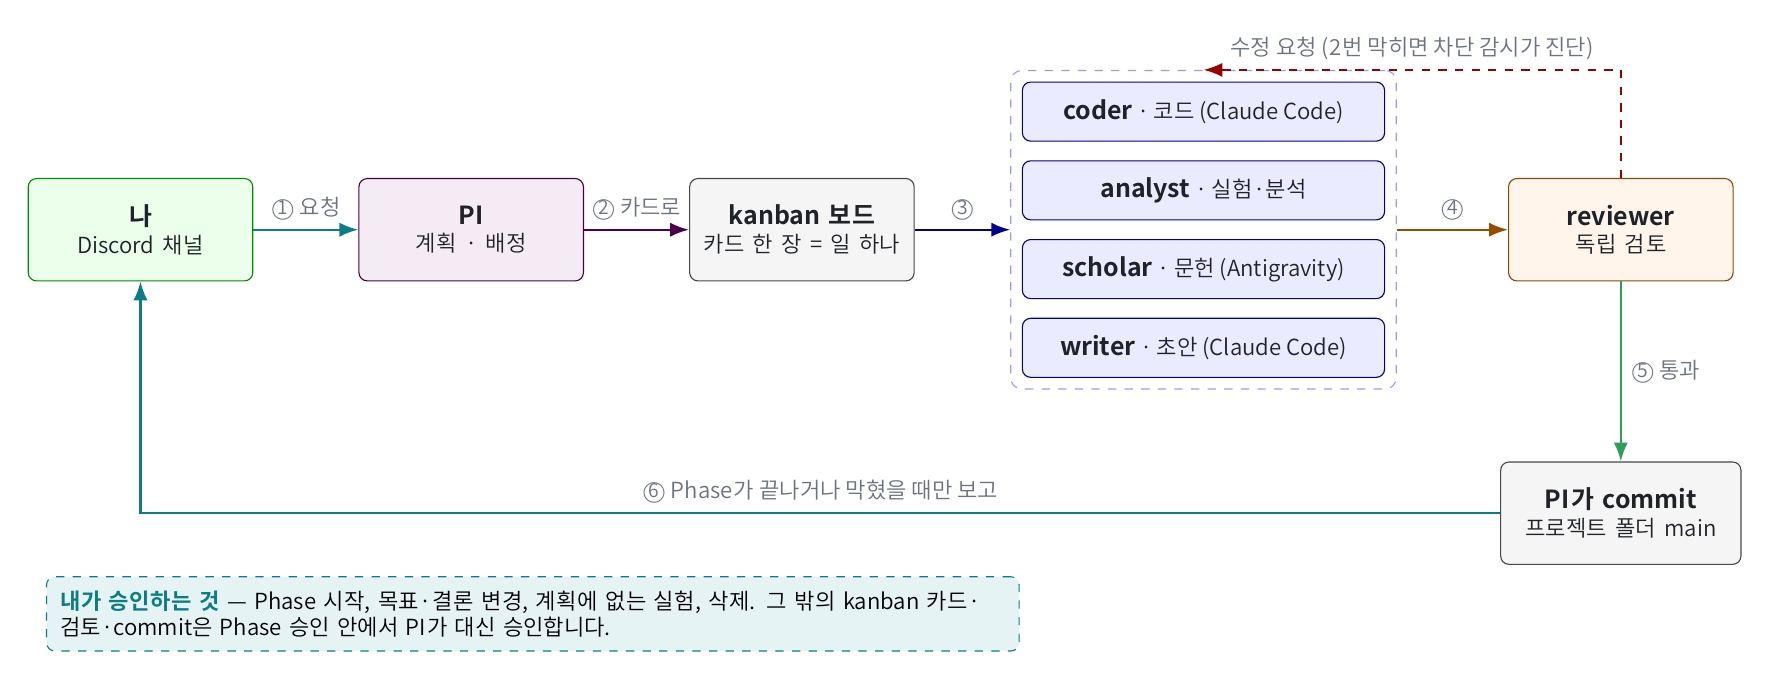
\includegraphics[width=\linewidth]{docs/figures/flow.png}
\end{center}
\begin{enumerate}
\item 내가 프로젝트 채널에서 PI에게 요청합니다.
\item PI가 일을 \textbf{kanban 카드}로 나눠 kanban 보드에 올리고 담당 직원을 정합니다.
\item 각 직원이 자기 kanban 카드를 실행합니다. coder·writer는 Claude Code로, scholar는 Antigravity로 실제 작업을 합니다.
\item 결과는 reviewer가 독립적으로 검토합니다. 문제가 있으면 수정 요청이 돌아가고, 같은 kanban 카드가 2번 막히면 자동 장치(차단 감시)가 원인을 진단합니다.
\item 통과하면 PI가 프로젝트 폴더의 \cmd{main}에 commit합니다.
\item PI는 Phase가 끝나거나 막혔을 때만 나에게 보고합니다.
\end{enumerate}

\section{준비물}

\begin{center}
\small
\begin{tabular}{L{0.22\linewidth} L{0.3\linewidth} L{0.38\linewidth}}
\toprule
\head \textbf{항목} & \textbf{어디에 쓰나} & \textbf{비고} \\
\midrule
Linux 서버 (예: \cmd{gnode1}) & 연구실 전체가 도는 곳 & SSH로 접속해 로그인 서버처럼 씁니다. 인터넷, 내 계정, 로컬 디스크의 홈 \cmd{/ai/works/<계정>} \\
로컬 모델 서버 & PI·coder·writer·scholar의 두뇌 & \textbf{이미 설치되어 있다고 가정합니다.} 주소(포트)만 알면 됩니다 \\
ChatGPT 구독 (Plus/Pro) & analyst·reviewer의 두뇌, 대화 압축 요약 & Hermes에서 \textbf{OpenAI → ChatGPT/Codex subscription}으로 로그인 \\
Claude 구독 (Pro/Max) & coder·writer의 작성 도구 Claude Code, 6명의 예비 모델 & 주 모델이 꺼지거나 한도에 걸리면 Claude Opus로 넘어갑니다 \\
Google 계정 & scholar의 논문 읽기 도구 Antigravity & \\
Discord 계정 + 내 서버 & 직원들과 대화하는 곳 & 서버 관리자여야 합니다. 없으면 3장에서 만듭니다 \\
메모장 & ID와 토큰 기록 & 1.6절의 기록표를 채웁니다 \\
\bottomrule
\end{tabular}
\end{center}

\info{걸리는 시간}{처음이면 2\textasciitilde3시간입니다. 대부분은 Discord 봇 6개를 만드는 시간(4장)입니다.
중간에 쉬어도 됩니다. 각 절 끝의 ``성공하면'' 상자를 확인하고 넘어가면 어디서 멈췄는지 알 수 있습니다.}

\subsection*{검증된 버전}
이 문서는 아래 버전에서 끝까지 확인했습니다. 더 새 버전이어도 대개 동작합니다. 명령이 바뀐 것 같으면 \cmd{<도구> --help}로 확인합니다.

\begin{center}
\small
\begin{tabular}{l l}
\toprule
\head \textbf{도구} & \textbf{버전} \\
\midrule
Hermes Agent & v0.22.5 (2026.9.24, stable) \\
Claude Code & 2.1.311 \\
Antigravity CLI (\cmd{agy}) & 1.4.7 \\
uv & 0.13.5 \\
git & 2.55.0 \\
\bottomrule
\end{tabular}
\end{center}

\section{이 문서를 읽는 법}

본문에는 다음 상자들이 나옵니다.

\begin{sh}
# 남색 상자: 터미널에 그대로 입력하는 명령. # 뒤는 설명이라 입력하지 않아도 된다
hermes --version
\end{sh}

\begin{filebox}{파일 이름}
\begin{code}
흰 상자: 파일에 적는 내용입니다. 제목 줄이 파일 이름입니다.
\end{code}
\end{filebox}

\begin{out}
회색 상자: 화면에 나오는 결과 예시입니다. 숫자나 날짜는 조금 달라도 됩니다.
\end{out}

\begin{msg}
보라색 상자: Discord 채널에 보내는 메시지입니다.
\end{msg}

\tip{팁}{알아 두면 편한 요령입니다.}
\warn{주의}{실수하기 쉬운 부분이나 비밀 정보 관련 주의 사항입니다.}
\ok{여기 적힌 결과가 나오면 그 절은 끝입니다. 다음으로 넘어갑니다.}

\textbf{꺾쇠 \cmd{<...>}는 내 값으로 바꿔 넣는 자리입니다.} 예를 들어 \cmd{<내이름>}은 \cmd{minji}처럼 바꿔 입력합니다. 꺾쇠 기호 자체는 지웁니다.

\section{터미널 기초 (처음이라면)}

이 매뉴얼의 명령은 모두 \textbf{터미널}에 입력합니다. Ubuntu에서는 \kbd{Ctrl}+\kbd{Alt}+\kbd{T}로 열립니다.
다른 컴퓨터에서 SSH로 접속해 작업해도 똑같습니다.

\begin{center}
\small
\begin{tabular}{L{0.3\linewidth} L{0.6\linewidth}}
\toprule
\head \textbf{하고 싶은 것} & \textbf{방법} \\
\midrule
명령 붙여 넣기 & \kbd{Ctrl}+\kbd{Shift}+\kbd{V} (터미널에서는 \kbd{Ctrl}+\kbd{V}가 아닙니다) \\
명령 실행 & \kbd{Enter}. 여러 줄을 한꺼번에 붙여 넣으면 차례로 실행됩니다 \\
실행 중인 것 멈추기 & \kbd{Ctrl}+\kbd{C} \\
이전 명령 다시 부르기 & \kbd{↑} \\
\cmd{~} 의 뜻 & 내 홈 폴더 (gnode1에서는 \cmd{/ai/works/<사용자>}) \\
\cmd{sudo} 비밀번호 & 내 로그인 비밀번호. 입력해도 화면에 \textbf{아무것도 표시되지 않는 것이 정상}입니다 \\
\bottomrule
\end{tabular}
\end{center}

\subsection*{nano로 파일 고치기}
설정 파일은 \cmd{nano}라는 간단한 편집기로 고칩니다. \cmd{nano <파일>}로 열고, 화살표 키로 움직여 고칩니다.

\begin{center}
\small
\begin{tabular}{l l}
\toprule
\head \textbf{키} & \textbf{동작} \\
\midrule
\kbd{Ctrl}+\kbd{O} 다음 \kbd{Enter} & 저장 \\
\kbd{Ctrl}+\kbd{X} & 나가기 \\
\kbd{Ctrl}+\kbd{K} & 지금 줄 잘라내기 (여러 번 누르면 여러 줄) \\
\kbd{Ctrl}+\kbd{W} & 찾기 \\
\kbd{Ctrl}+\kbd{Shift}+\kbd{V} & 붙여 넣기 \\
\bottomrule
\end{tabular}
\end{center}

\section{ID 기록표}

설치하는 동안 Discord ID 10여 개와 봇 토큰 6개가 나옵니다. 아래 표를 메모장에 복사해 두고 채워 나갑니다.

\begin{filebox}{메모장 (내 컴퓨터에만 보관)}
\begin{code}
[Discord]
서버(guild) ID         :
로비 채널(#hermes) ID  :
Projects 카테고리 ID   :
내 사용자 ID           :

[봇]                    Application ID       봇(사용자) ID        토큰(비밀)
PI (hermes-researcher) :
coder                  :
analyst                :
reviewer               :
writer                 :
scholar                :
\end{code}
\end{filebox}

\warn{토큰은 비밀번호입니다}{봇 토큰을 가진 사람은 그 봇으로 무엇이든 할 수 있습니다.
채팅·메일·git·스크린샷에 올리지 마세요. 실수로 노출됐다면 Discord 개발자 페이지에서 \textbf{Reset Token}으로 새로 만듭니다.}

\info{두 가지 경우}{이 문서는 \textbf{새 연구실을 처음 만드는 경우}입니다.
이미 돌고 있는 연구실을 다른 컴퓨터로 \emph{옮기는} 경우는 부록~\ref{app:move}만 따라 합니다.
같은 봇 토큰을 두 컴퓨터에서 동시에 쓰면 나중에 켠 쪽이 연결에 실패합니다.}

\section{설치 위치 확인: 홈이 /ai/works에 있는지}
\label{sec:where}
\does{작업 서버(gnode1)에서 내 홈 폴더가 그 서버의 로컬 디스크에 잡혀 있는지 확인합니다. \textbf{도구를 설치하기 전에} 해야 합니다.}

이 연구실은 클러스터의 계산 노드 \cmd{gnode1}을 \textbf{두 번째 로그인 서버처럼} 씁니다. 로그인 서버를 거치지 않고 내 PC에서 gnode1(\cmd{172.27.120.13})로 바로 SSH 접속해 설치하고, Hermes도 gnode1에서만 돌립니다.
클러스터에는 성격이 다른 디스크가 여럿 있으니 먼저 지도를 봅니다.

\begin{center}
\small
\begin{tabular}{L{0.3\linewidth} L{0.24\linewidth} L{0.36\linewidth}}
\toprule
\head \textbf{경로} & \textbf{어디에 있나} & \textbf{이 연구실에서의 쓰임} \\
\midrule
\cmd{/ai/works/<계정>} & gnode1 로컬 디스크 & \textbf{gnode1에서의 내 홈(\cmd{~})}. Hermes(\cmd{~/.hermes}), 프로젝트(\cmd{~/Projects}) 모두 여기 \\
\cmd{/data/datasets} & gnode1 로컬 디스크 & 연구실 공용 데이터셋 \\
\cmd{/data/<계정>} & gnode1 로컬 디스크 & 계산 노드에서 돌린 실험 결과가 도착하는 곳 (\ref{sec:hpc}절) \\
\cmd{/home/<계정>} & 로그인 서버의 공유 디스크(NFS) & 다른 노드에서의 홈. gnode1에서는 계산 노드로 파일을 보낼 때 \textbf{잠깐 거쳐 가는 곳}으로만 씁니다 \\
\bottomrule
\end{tabular}
\end{center}

공유 디스크(NFS)에 Hermes를 두지 않는 이유는 두 가지입니다.
\begin{itemize}
\item Hermes는 대화 기록과 kanban 보드를 데이터베이스 파일로 씁니다. 공유 디스크에서는 이 파일이 잠기거나(\cmd{database is locked}) 느려질 수 있습니다.
\item 공유 디스크는 모든 노드가 같이 쓰므로, 프로젝트의 Python 환경(\cmd{.venv})처럼 큰 파일을 두면 다른 사람까지 느려집니다.
\end{itemize}
gnode1에서는 관리자가 로그인할 때 홈을 \cmd{/ai/works/<계정>}으로 바꿔 주도록 설정해 두었습니다. 그래서 이 문서의 \cmd{~/.hermes}, \cmd{~/Projects}는 그대로 \cmd{/ai/works/<계정>/} 아래가 됩니다. 링크를 만들거나 스크립트를 고칠 필요가 없습니다.

\subsection{gnode1에 접속하고 홈 위치 확인}
gnode1에는 로그인 서버를 거치지 않고 \textbf{내 PC에서 바로} 접속합니다. 주소는 \cmd{172.27.120.13}이고, 포트 번호는 관리자에게 물어봅니다.
내 PC의 터미널(Windows는 PowerShell)에서 \cmd{<포트>}와 \cmd{<계정>}을 바꿔 실행합니다.
\begin{sh}
ssh -p <포트> <계정>@172.27.120.13
\end{sh}
처음 접속하면 \cmd{Are you sure you want to continue connecting}이 나옵니다. \cmd{yes}를 입력하고 비밀번호를 넣습니다.
\textbf{이후 이 문서의 모든 명령은 gnode1에서} 실행합니다. 접속했으면 홈 위치를 확인합니다.
\begin{sh}
echo $HOME
df -hT $HOME
\end{sh}
\begin{out}
/ai/works/minji
Filesystem     Type  Size  Used Avail Use% Mounted on
/dev/sdb1      ext4   15T  2.1T   13T  15% /ai
\end{out}
\ok{\cmd{echo $HOME}이 \cmd{/ai/works/<계정>}이고, \cmd{df}의 Type이 \cmd{ext4}나 \cmd{xfs}(로컬 디스크)입니다.}
\warn{\cmd{/home/<계정>}이 나오면}{gnode1의 홈 설정이 아직 안 된 계정입니다. 관리자에게 \cmd{/ai/works/<계정>} 폴더와 홈 설정을 부탁합니다.}
\tip{매번 주소와 포트를 치기 귀찮다면}{\textbf{내 PC}의 \cmd{~/.ssh/config} 파일에 아래 네 줄을 넣으면 그다음부터는 \cmd{ssh gnode1}만 치면 됩니다.\par
\cmd{Host gnode1}\par
\cmd{HostName 172.27.120.13}\par
\cmd{Port <포트>}\par
\cmd{User <계정>}}

\subsection{로그인 설정 파일 챙기기}
새 홈은 비어 있어서, 로그인할 때 읽는 설정 파일이 없을 수 있습니다. 특히 \cmd{.profile}이 없으면 \cmd{.bashrc}가 자동으로 읽히지 않아 매번 \cmd{source ~/.bashrc}를 해야 합니다.
\begin{sh}
ls -a ~
\end{sh}
\cmd{.profile}이나 \cmd{.bashrc}가 없으면 기본 파일을 복사합니다. \cmd{-n}은 ``이미 있으면 덮어쓰지 않는다''는 뜻입니다.
\begin{sh}
cp -n /etc/skel/.profile /etc/skel/.bashrc ~/
\end{sh}
로그인 서버에서 쓰던 \cmd{.bashrc}(별칭, conda 설정 등)를 그대로 쓰고 싶다면 대신 그것을 복사합니다.
\begin{sh}
cp /home/$USER/.bashrc ~/.bashrc
\end{sh}
SSH를 끊었다가 다시 접속합니다.
\begin{sh}
exit
ssh -p <포트> <계정>@172.27.120.13
grep -c bashrc ~/.profile
\end{sh}
\ok{숫자가 1 이상이면 \cmd{.profile}이 \cmd{.bashrc}를 읽습니다. 이제 \cmd{source ~/.bashrc} 없이도 설정이 적용됩니다.}

\subsection{서비스용 홈 확인}
\label{sec:svchome}
Hermes 게이트웨이는 \textbf{systemd 사용자 서비스}로 등록해, SSH를 끊거나 서버가 재부팅돼도 계속 돌게 합니다(\ref{sec:gwservice}절).
그러려면 gnode1이 내 홈을 \cmd{/ai/works/<계정>}으로 알고 있어야 합니다. 관리자가 미리 설정해 두었는지 세 가지를 확인합니다.
\begin{sh}
getent passwd $USER
systemctl --user show -p UnitPath | tr ' ' '\n' | grep -c works
loginctl show-user $USER -p Linger
\end{sh}
\begin{out}
minji:x:1023:1023:,,,:/ai/works/minji:/bin/bash
3
Linger=yes
\end{out}
\ok{첫 줄 끝이 \cmd{/ai/works/<계정>:/bin/bash}, 둘째 줄이 \cmd{1} 이상, 셋째 줄이 \cmd{Linger=yes}입니다. 이 문서는 이 상태를 기준으로 씁니다.}
\warn{하나라도 다르면}{설치는 그대로 진행해도 됩니다(2\textasciitilde5장은 로그인 셸에서만 합니다). 다만 게이트웨이를 서비스로 등록하기 전에 \ref{sec:gwfix}절 순서대로 관리자에게 부탁해 고칩니다.
첫 줄은 맞는데 둘째 줄만 \cmd{0}이면 관리자 없이 해결됩니다: \cmd{systemctl --user exit} 후 SSH를 모두 끊고 다시 접속합니다.}

\warn{Hermes는 gnode1에서만 켭니다}{다른 노드에서는 홈이 \cmd{/home/<계정>}이라 \cmd{~/.hermes}가 없습니다. 다른 서버에서 \cmd{hermes}를 설치하거나 실행하지 마세요.
같은 봇 토큰으로 게이트웨이가 두 개 뜨면 나중에 켠 쪽이 연결에 실패합니다.}

\tip{로컬 디스크는 백업되지 않는 경우가 많습니다}{디스크가 고장 나면 사라집니다. 연구 프로젝트는 git 원격 저장소에 push해 두고,
가끔 \cmd{hermes backup}(부록~\ref{app:move})과 \cmd{bash tools/memories.sh export}로 설정과 기억을 받아 둡니다.}

% ================================================================
\chapter{기본 도구 설치}

이 장에서는 터미널에서 도구 다섯 개를 설치하고 각자 로그인합니다. 모두 \textbf{일반 사용자}로 실행합니다.
\cmd{sudo}는 쓰라고 한 곳에서만 씁니다.

\section{기본 패키지와 git}
\does{설치 스크립트를 받는 \cmd{curl}, 버전 관리 \cmd{git}, 스크립트를 돌리는 \cmd{python3}를 준비합니다.}
\begin{sh}
git --version && curl --version | head -1 && python3 --version
\end{sh}
세 줄 모두 버전이 나오면 이미 설치된 것이므로 넘어갑니다. 하나라도 \cmd{command not found}이면 설치합니다.
\begin{sh}
sudo apt update && sudo apt install -y git curl python3
\end{sh}
\tip{공용 서버에서 sudo 권한이 없다면}{관리자에게 설치를 부탁합니다. 이 문서에서 \cmd{sudo}가 필요한 곳은 여기와 \ref{sec:svchome}절(gnode1 홈 설정, linger) 두 곳뿐입니다.}

이어서 git에 내 이름을 알려 줍니다. 직원들이 만드는 commit에 이 이름이 남습니다.
\begin{sh}
git config --global user.name  "<이름>"
git config --global user.email "<이메일>"
git config --global init.defaultBranch main
\end{sh}
마지막 줄은 새 저장소의 기본 브랜치를 \cmd{master}가 아니라 \cmd{main}으로 만듭니다. 직원들은 \cmd{main}을 기준으로 일하므로 꼭 넣습니다.

\ok{\cmd{git config --global --list}에 이름·이메일·\cmd{init.defaultbranch=main}이 보입니다.}

\section{uv (프로젝트별 Python 환경)}
\does{프로젝트마다 Python 패키지를 따로 관리하는 도구를 설치합니다. 새 프로젝트를 만들 때 직원들이 씁니다.}
\begin{sh}
curl -LsSf https://astral.sh/uv/install.sh | sh
source ~/.bashrc
uv --version
\end{sh}
\ok{\cmd{uv 0.13.5}처럼 버전이 나옵니다.}

\subsection*{conda를 쓰던 사람을 위한 uv}
uv는 \textbf{프로젝트 폴더마다 conda 환경이 하나씩 붙어 있는 것}이라고 보면 됩니다. 이 연구실의 프로젝트는 conda 대신 uv를 씁니다.
\begin{center}
\small
\begin{tabular}{L{0.24\linewidth} L{0.32\linewidth} L{0.34\linewidth}}
\toprule
\head \textbf{하고 싶은 일} & \textbf{conda} & \textbf{uv (프로젝트 폴더에서)} \\
\midrule
환경 만들기 & \cmd{conda create -n myenv} & \cmd{uv init} (환경은 폴더 안 \cmd{.venv/}) \\
패키지 설치·제거 & \cmd{conda install} / \cmd{remove} & \cmd{uv add} / \cmd{uv remove} \\
환경에서 실행 & \cmd{conda activate} 후 \cmd{python} & \cmd{uv run python a.py} \\
켜 두고 계속 쓰기 & \cmd{conda activate myenv} & \cmd{source .venv/bin/activate} \\
패키지 목록 저장 & \cmd{environment.yml} (직접 export) & \cmd{pyproject.toml}, \cmd{uv.lock} (자동) \\
환경 지우기 & \cmd{conda env remove -n myenv} & \cmd{rm -rf .venv} (\cmd{uv sync}로 다시 만듦) \\
\bottomrule
\end{tabular}
\end{center}
한 프로젝트에서 패키지를 바꿔도 다른 프로젝트는 영향을 받지 않습니다. 한 번 받은 패키지는 캐시에 남아 다시 설치할 때 몇 초면 됩니다.
\cmd{uv.lock}에 정확한 버전이 적혀 있어서, 계산 노드에도 같은 환경을 옮길 수 있습니다(\ref{sec:hpc}절).
\tip{conda가 저절로 켜지지 않게}{프롬프트 앞에 \cmd{(base)}가 보이면 conda가 켜진 상태라 uv 환경과 섞일 수 있습니다. \cmd{conda config --set auto_activate_base false}로 꺼 둡니다. conda는 그대로 남고, 필요할 때 \cmd{conda activate}로 직접 켭니다. 직원들은 conda를 건드리지 않습니다.}

\section{Hermes Agent}
\does{직원들의 몸체인 Hermes Agent를 설치합니다.}
\begin{sh}
curl -fsSL https://hermes-agent.nousresearch.com/install.sh | bash -s -- --non-interactive
source ~/.bashrc
hermes --version
\end{sh}
\cmd{--non-interactive}는 설치가 끝난 뒤 자동으로 뜨는 설정 마법사와 게이트웨이 서비스 등록을 건너뛰라는 뜻입니다.
모델 설정은 \ref{sec:pisetup}절, 서비스 등록은 \ref{sec:gwservice}절에서 따로 하므로 여기서는 프로그램만 설치합니다.
설치되면 세 곳에 파일이 생깁니다.
\begin{itemize}
\item \cmd{~/.hermes/hermes-agent/}: 프로그램 코드
\item \cmd{~/.local/bin/hermes}: 명령
\item \cmd{~/.hermes/}: 설정, 토큰, 대화 기록 (\textbf{비밀 포함})
\end{itemize}

\warn{\cmd{How would you like to set up Hermes?} 창이 떴다면}{\cmd{--non-interactive} 없이 설치한 경우입니다. 아무것도 고르지 말고 \kbd{Ctrl}+\kbd{C}를 눌러 명령 프롬프트로 돌아옵니다(한 번에 안 나가면 몇 번 더).
그다음 위의 \cmd{curl} 줄을 그대로 다시 실행합니다. 이미 받은 파일은 건너뛰고 빠르게 끝납니다.
목록 첫 줄의 \textbf{Quick Setup (Nous Portal)}은 별도 유료 서비스 로그인이라 이 연구실에서는 쓰지 않습니다.}

\tip{\cmd{hermes: command not found}가 나오면}{\cmd{source ~/.bashrc}를 한 번 더 하거나, 터미널을 닫고 새로 엽니다.
그래도 안 되면 \cmd{echo 'export PATH="$HOME/.local/bin:$PATH"' >> ~/.bashrc} 후 다시 \cmd{source ~/.bashrc}.}

\ok{\cmd{hermes --version}이 \cmd{v0.22.5} 이상을 출력합니다.}

\section{Claude Code}
\does{coder·writer가 실제 코드와 글을 쓸 때 부르는 도구를 설치하고 Claude 구독 계정으로 로그인합니다.}
\begin{sh}
curl -fsSL https://claude.ai/install.sh | bash
source ~/.bashrc
claude
\end{sh}

처음 실행하면 다음 순서로 진행됩니다.
\begin{enumerate}
\item 화면 테마를 고릅니다 (아무거나).
\item 로그인 방법에서 \textbf{Claude 구독 계정(Pro/Max)}을 고릅니다.
\item 브라우저가 열리면 로그인하고 승인합니다. 브라우저가 없는 컴퓨터(SSH 접속)라면 화면에 나온 주소를 복사해 \emph{내 컴퓨터의} 브라우저에 붙여 넣고,
  승인 후 나오는 코드를 터미널의 \cmd{Paste code here} 자리에 붙여 넣습니다.
\item ``이 폴더를 신뢰하겠냐''고 물으면, 지금은 홈 폴더(\cmd{~})에서 열었으므로 \textbf{No}를 고릅니다.
\item \cmd{/exit}를 입력해 나옵니다.
\end{enumerate}

이제 직원들이 쓰는 방식(\cmd{claude -p})으로 한 번 시험합니다.
\begin{sh}
claude -p "OK라고만 답해" --max-turns 1
\end{sh}
\begin{out}
OK
\end{out}

\warn{\cmd{ANTHROPIC_API_KEY}가 설정되어 있다면}{\cmd{~/.bashrc}에 \cmd{ANTHROPIC_API_KEY}가 있으면 구독 대신 API 요금으로 청구됩니다.
구독으로 쓰려면 그 줄을 지우고 \cmd{unset ANTHROPIC_API_KEY} 후 다시 실행합니다.}

\ok{마지막 명령이 \cmd{OK}를 출력합니다.}

\section{Antigravity CLI}
\does{scholar가 논문 웹 페이지를 읽을 때 쓰는 도구를 설치하고 Google 계정으로 로그인합니다.}
\begin{sh}
curl -fsSL https://antigravity.google/cli/install.sh | bash
source ~/.bashrc
agy --version
\end{sh}
공식 설치 스크립트가 \cmd{agy} 파일 하나를 \cmd{~/.local/bin/}에 넣습니다. \cmd{agy: command not found}가 나오면 2.3절 팁처럼 PATH를 확인합니다.

이어서 \cmd{agy}를 한 번 실행해 Google 계정으로 로그인한 뒤 나옵니다. SSH로 접속해 브라우저가 열리지 않으면, 화면에 나온 주소를 내 PC 브라우저에 붙여 넣어 로그인합니다.
\begin{sh}
agy
\end{sh}
로그인했으면 동작을 확인합니다.
\begin{sh}
agy -p "Reply with OK" --output-format json --print-timeout 2m
\end{sh}
\begin{out}
{ ... "status": "SUCCESS", ... }
\end{out}
읽기 권한(어떤 사이트를 읽어도 되는지)은 6장에서 한 번에 설정합니다.

\ok{출력 JSON의 \cmd{"status"}가 \cmd{"SUCCESS"}입니다.}

\section{연구실 설정 묶음 가져오기}
\does{직원들의 역할·규칙과 설치 도우미 스크립트가 든 \cmd{hermes-team} 폴더를 정해진 위치에 받습니다.}

위치는 반드시 \cmd{~/Projects/hermes-team}입니다. 스크립트들이 이 경로를 기준으로 동작합니다.
\begin{sh}
mkdir -p ~/Projects && cd ~/Projects
git clone https://github.com/<저장소>.git hermes-team
ls ~/Projects/hermes-team
\end{sh}
\begin{out}
docs  extras  INSTALL.md  install_souls.sh  LOCAL_MODEL.md  newproject.py  README.md
set_name.sh  SETUP.md  souls  template  tools
\end{out}

\tip{GitHub 대신 파일로 받았다면}{\cmd{hermes-team-share.tar}를 받았다면 \cmd{tar xf hermes-team-share.tar -C ~/Projects}로 풀고
폴더 이름을 \cmd{hermes-team}으로 바꿉니다 (\cmd{mv ~/Projects/hermes-team-share ~/Projects/hermes-team}).}

\subsection{연구자 이름 정하기}
직원들은 나를 이름으로 부르고 승인을 요청합니다. 원본 규칙 파일에는 이름 자리가 \cmd{{{연구자}}}로 비어 있고, 아래 명령이 내 이름으로 채웁니다.
\begin{sh}
cd ~/Projects/hermes-team
bash set_name.sh <내이름>        # 예: minji 또는 김민지 (공백 없이)
\end{sh}
이 명령은 \textbf{내 컴퓨터 전용 설정 파일} 세 개(\cmd{team.json}, \cmd{souls/_team_ids.md}, \cmd{projects.json})를 예시에서 만들고,
commit할 때 개인 정보가 섞이지 않게 막는 검사를 켭니다. 이 세 파일은 git에 올라가지 않습니다. 나중에 다시 실행해도 됩니다.

\ok{\cmd{다음: INSTALL.md 를 처음부터 따라 한다.}가 출력되고, \cmd{ls team.json souls/_team_ids.md projects.json}에 세 파일이 모두 보입니다.}

% ================================================================
\chapter{Discord 서버 준비}

\section{개발자 모드 켜기}
\does{Discord에서 서버·채널·사용자의 ID를 복사할 수 있게 합니다.}

Discord 앱(PC 권장) → 왼쪽 아래 \textbf{사용자 설정(톱니바퀴)} → \textbf{고급} → \textbf{개발자 모드} 켜기.

이제 서버, 채널, 사용자를 \textbf{우클릭}하면 메뉴 맨 아래에 \textbf{ID 복사}가 나옵니다.

\section{서버와 채널 만들기}
연구실 전용 서버가 없다면 왼쪽 서버 목록의 \textbf{+} → \textbf{직접 만들기} → \textbf{나와 친구들을 위한 서버}로 만듭니다.
그 서버 안에 다음을 만듭니다.

\begin{center}
\small
\begin{tabular}{L{0.2\linewidth} L{0.17\linewidth} L{0.53\linewidth}}
\toprule
\head \textbf{만들 것} & \textbf{이름} & \textbf{용도} \\
\midrule
텍스트 채널 & \ch{hermes} & \textbf{로비.} 전체 상황, 새 프로젝트 요청. PI가 멘션 없이 답합니다 \\
카테고리 & \cmd{Projects} & PI가 프로젝트 채널을 \textbf{자동으로} 이 안에 만듭니다 \\
텍스트 채널 (선택) & \ch{sandbox} & 시험용 \\
\bottomrule
\end{tabular}
\end{center}

채널은 채널 목록의 \textbf{+} 버튼, 카테고리는 서버 이름 클릭 → \textbf{카테고리 만들기}로 만듭니다.

\section{ID 네 개 복사하기}
아래 네 곳을 우클릭 → \textbf{ID 복사}로 복사해 기록표에 붙여 넣습니다.

\begin{center}
\small
\begin{tabular}{L{0.35\linewidth} L{0.55\linewidth}}
\toprule
\head \textbf{우클릭할 곳} & \textbf{기록표 칸} \\
\midrule
왼쪽 목록의 서버 아이콘 & 서버(guild) ID \\
\ch{hermes} 채널 & 로비 채널 ID \\
\cmd{Projects} 카테고리 이름 & Projects 카테고리 ID \\
채팅창의 내 프로필(이름) & 내 사용자 ID \\
\bottomrule
\end{tabular}
\end{center}

\ok{기록표의 [Discord] 네 칸이 모두 18\textasciitilde19자리 숫자로 채워졌습니다.}

% ================================================================
\chapter{직원 6명 만들기}

직원 한 명은 \textbf{Discord 봇 하나}와 \textbf{Hermes profile 하나}로 이루어집니다.

\begin{center}
\small
\begin{tabular}{l l l}
\toprule
\head \textbf{직원} & \textbf{Discord 봇 이름} & \textbf{Hermes profile} \\
\midrule
PI & \cmd{hermes-researcher} & \cmd{default} (기본 profile) \\
coder & \cmd{coder} & \cmd{coder} \\
analyst & \cmd{analyst} & \cmd{analyst} \\
reviewer & \cmd{reviewer} & \cmd{reviewer} \\
writer & \cmd{writer} & \cmd{writer} \\
scholar & \cmd{scholar} & \cmd{scholar} \\
\bottomrule
\end{tabular}
\end{center}

\section{Discord 봇 6개 만들기}
\does{Discord 개발자 페이지에서 봇을 만들고, 토큰을 받고, 내 서버에 초대합니다. 아래 1\textasciitilde5를 \textbf{봇마다 반복}합니다 (6번).}

\begin{enumerate}[label=\textbf{\arabic*.}]
\item 브라우저에서 \href{https://discord.com/developers/applications}{\cmd{https://discord.com/developers/applications}}를 열고 Discord 계정으로 로그인합니다.
  오른쪽 위 \textbf{New Application} → 이름 입력(위 표의 봇 이름) → 약관 동의 체크 → \textbf{Create}.
\item 왼쪽 \textbf{General Information}에서 \textbf{Application ID}를 \textbf{Copy} → 기록표의 그 봇 줄 ``Application ID'' 칸.
\item 왼쪽 \textbf{Bot}을 누릅니다.
  \begin{itemize}
  \item \textbf{Reset Token} → 확인 → 나온 토큰을 \textbf{Copy} → 기록표 ``토큰'' 칸. \textbf{이 화면을 벗어나면 다시 볼 수 없습니다.}
  \item 아래로 내려 \textbf{Privileged Gateway Intents}의 \textbf{Message Content Intent}를 켭니다 → 아래쪽 \textbf{Save Changes}.
  \end{itemize}
\item 서버에 초대합니다. 브라우저 주소창에 아래 주소를 붙여 넣되, 끝의 \cmd{APP_ID}를 2번에서 복사한 값으로 바꿉니다.
\begin{sh}[fontsize=\footnotesize]
https://discord.com/oauth2/authorize?scope=bot+applications.commands&permissions=274878024768&client_id=APP_ID
\end{sh}
  승인 화면 위쪽에 나온 봇 이름이 \textbf{지금 만드는 봇인지} 확인 → 서버 선택에서 내 연구실 서버 → \textbf{계속하기} → \textbf{승인}.
\item Discord 앱으로 돌아와 서버 오른쪽 멤버 목록에서 방금 들어온 봇을 우클릭 → \textbf{ID 복사} → 기록표 ``봇 ID'' 칸.
\end{enumerate}

\warn{Message Content Intent를 꼭 켜세요}{꺼져 있으면 봇이 메시지를 읽지 못해 게이트웨이가 접속에 실패합니다. 가장 흔한 실수입니다.}
\tip{Application ID와 봇 ID}{둘은 보통 같은 숫자입니다. 다르게 나와도 괜찮습니다. 기록표에는 각각 적어 둡니다.
나중에 쓰는 것은 \textbf{봇 ID}(5번)입니다.}

\ok{서버 멤버 목록에 봇 6개(\cmd{hermes-researcher}, \cmd{coder}, \cmd{analyst}, \cmd{reviewer}, \cmd{writer}, \cmd{scholar})가 오프라인으로 보이고,
기록표의 [봇] 표가 모두 채워졌습니다. 봇은 게이트웨이를 켜는 \ref{sec:gwservice}절에서 온라인이 됩니다.}

\section{PI 설정}
\label{sec:pisetup}
\does{PI(기본 profile)를 완성합니다. 주 모델은 로컬 모델, 예비 모델은 Claude로 정하고 PI 봇 토큰을 넣습니다.}

이 절은 \textbf{로컬 모델 서버가 이미 돌고 있다}는 전제에서 시작합니다. 아직 설치하지 않았다면 \cmd{LOCAL_MODEL.md}(또는 \cmd{LOCAL_MODEL.pdf})를 먼저 따라 하고 돌아옵니다.

PI를 먼저 완성하는 이유는 4.3절에서 나머지 5명을 \textbf{PI를 복제해} 만들기 때문입니다. 여기서 정한 모델과 예비 모델이 그대로 복사되므로, 다섯 명에게는 봇 토큰을 넣고 analyst·reviewer만 ChatGPT로 바꾸면 됩니다.

\subsection{로컬 모델 서버 확인}
\label{sec:modelcheck}
포트는 모델 서버를 설치한 방식에 따라 다릅니다.
\begin{itemize}
\item \textbf{개인 데스크탑}: \cmd{8080}
\item \textbf{공용 서버}: 관리자에게 배정받은 포트 (\cmd{8081}\textasciitilde\cmd{8085} 중 하나)
\end{itemize}
포트 번호를 \cmd{~/.bashrc}에 \cmd{LLAMA_PORT}라는 이름으로 적어 둡니다. 그러면 터미널을 새로 열어도 \cmd{$LLAMA_PORT}라고 쓴 곳이 그 숫자로 바뀝니다.
첫 줄의 \cmd{8081} 자리에 \textbf{내 포트 숫자}를 넣어 실행합니다 (\cmd{=} 앞뒤에 띄어쓰기 없이).
\begin{sh}
echo 'export LLAMA_PORT=8081' >> ~/.bashrc
source ~/.bashrc
echo $LLAMA_PORT
curl -s http://127.0.0.1:$LLAMA_PORT/v1/models
\end{sh}
\begin{out}
{"object":"list","data":[{"id":"qwen3.6-35b-a3b", ... }]}
\end{out}
\ok{출력에 \cmd{qwen3.6-35b-a3b}가 보입니다.}

\warn{아무것도 안 나오거나 \cmd{Connection refused}}{모델 서버가 꺼져 있습니다.
데스크탑은 \cmd{systemctl --user status llama-server}, 공용 서버는 \cmd{systemctl status llama-qwen@<번호>}로 상태를 보고,
\cmd{active (running)}이 아니면 \cmd{LOCAL_MODEL.md}의 해당 절을 다시 확인합니다.}
\tip{포트가 바뀌면}{\cmd{nano ~/.bashrc}로 맨 아래 \cmd{export LLAMA_PORT=} 줄의 숫자를 고치고, \ref{sec:changemain}절의 ``로컬 모델 포트가 바뀌었을 때'' 명령으로 직원들의 주소도 고칩니다.}

\subsection{주 모델을 로컬 모델로}
\label{sec:tolocal}
설정 파일(\cmd{config.yaml})은 2천 줄이 넘어서, 손으로 열어 고치면 실수하기 쉽습니다.
그래서 파일을 직접 열지 않고 \cmd{hermes config set <항목> <값>} 명령으로 필요한 줄만 바꿉니다. 다른 줄과 주석은 건드리지 않습니다.
첫 줄은 원본 설정을 \cmd{.before-local}로 백업합니다.
\begin{sh}
cp "$(hermes config path)" "$(hermes config path).before-local"
hermes config set model.default qwen3.6-35b-a3b
hermes config set model.provider custom:local-qwen
hermes config set model.context_length 131072
hermes config set providers.local-qwen.base_url http://127.0.0.1:$LLAMA_PORT/v1
hermes config set providers.local-qwen.default_model qwen3.6-35b-a3b
\end{sh}
\begin{out}
✓ Set model.default = qwen3.6-35b-a3b in /ai/works/minji/.hermes/config.yaml
✓ Set model.provider = custom:local-qwen in ...
...
\end{out}
\ok{다섯 줄 모두 \cmd{✓ Set}이 나옵니다.}

\begin{center}
\small
\begin{tabular}{L{0.38\linewidth} L{0.52\linewidth}}
\toprule
\head \textbf{항목} & \textbf{뜻} \\
\midrule
\cmd{model.default} & 쓸 모델 이름. 모델 서버의 \cmd{--alias}와 똑같아야 합니다 \\
\cmd{model.provider} & 어디로 보낼지. \cmd{custom:local-qwen}은 아래 \cmd{providers.local-qwen}을 쓰라는 뜻입니다 \\
\cmd{model.context_length} & 한 번에 읽는 문맥 길이. 모델 서버의 \textbf{슬롯 하나당} 길이(\cmd{131072})와 맞춥니다 \\
\cmd{providers.local-qwen.base_url} & 모델 서버 주소 \\
\bottomrule
\end{tabular}
\end{center}

\tip{되돌리기}{처음 상태로 되돌리려면 백업을 덮어씁니다. 예: \cmd{cp ~/.hermes/config.yaml.before-local ~/.hermes/config.yaml}
(직원은 \cmd{~/.hermes/profiles/<직원>/config.yaml.before-local})}

\subsection{예비 모델 넣기}
\label{sec:fallback}
주 모델이 실패하면 Claude가 대신 답하게 합니다.

\begin{center}
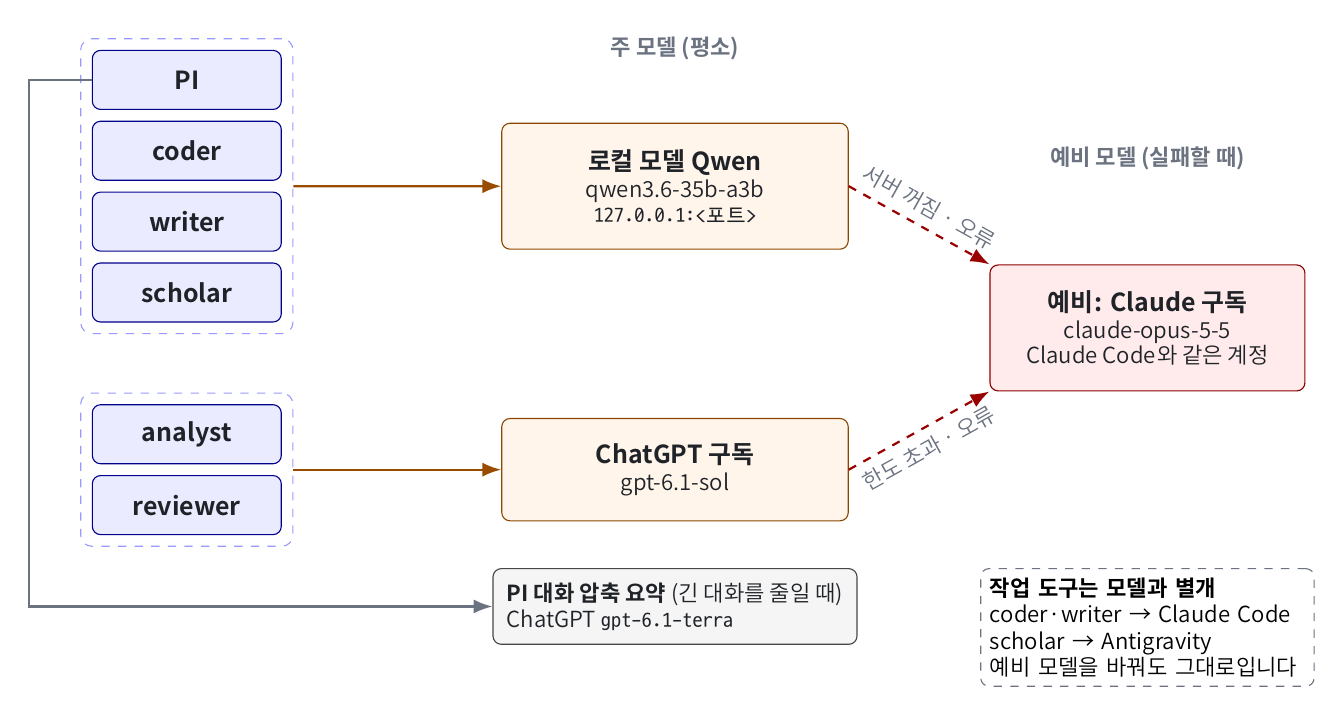
\includegraphics[width=\linewidth]{docs/figures/models.png}
\end{center}

예비 모델은 주 모델이 \textbf{꺼져 있거나, 오류를 내거나, 사용 한도에 걸렸을 때} 자동으로 쓰입니다.
\begin{itemize}
\item 로컬 모델 직원: 모델 서버가 꺼져 있거나 재시작 중일 때 Claude로 넘어갑니다.
\item analyst·reviewer: ChatGPT 사용 한도에 걸리면 Claude로 넘어갑니다.
\item Claude는 2.4절에서 로그인한 \textbf{Claude 구독}을 씁니다. 따로 로그인할 것은 없습니다.
\end{itemize}

Claude 구독으로 답하는 기능은 Hermes 기본 설치에 들어 있지 않고, Nous Research 공식 플러그인으로 따로 설치합니다.
2.4절에서 설치·로그인한 \cmd{claude} 명령을 통해 Claude 구독을 씁니다.
\begin{sh}
hermes plugins install claude-subscription-directsdk --enable
hermes plugins list | grep claude-subscription
\end{sh}
\ok{\cmd{claude-subscription-directsdk}가 \cmd{enabled}로 보입니다. 설치를 물으면 \cmd{y}로 답합니다.}
설치되면 \cmd{hermes model}의 provider 목록에도 아래 줄이 생깁니다 (여기서 고르지는 않습니다. 고르면 PI의 주 모델이 Claude로 바뀝니다).
\begin{center}
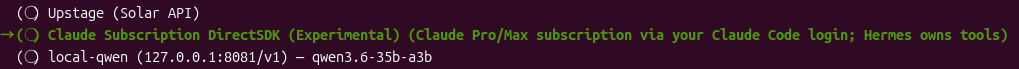
\includegraphics[width=\linewidth]{docs/figures/menu-claude.png}\par
{\footnotesize\color{muted} \textbf{Claude Subscription DirectSDK (Experimental)}: 예비 모델 설정에 쓰는 provider \cmd{claude-subscription-directsdk-experimental}}
\end{center}
\warn{\cmd{Unknown provider 'claude-subscription-directsdk-experimental'}이 나오면}{이 플러그인이 설치·활성화되지 않은 것입니다. 위 두 줄을 실행합니다.
PI에 설치한 뒤 4.3절에서 복제하면 직원들에게도 같이 들어갑니다.}

\textbf{고장 난 예비 모델은 오히려 해롭습니다.} 예비 모델까지 실패하면 진짜 실패로 세어지고, 같은 kanban 카드가 2번 실패하면 \cmd{blocked}가 됩니다.
그래서 넣기 전에 그 모델 하나만 따로 불러 봅니다.
\begin{sh}
hermes chat --provider claude-subscription-directsdk-experimental -m claude-opus-5-5 -q "OK라고만 답해"
\end{sh}
\ok{\cmd{OK}가 나옵니다. 오류가 나면 2.4절(Claude Code 로그인)부터 다시 확인하고, 통과할 때까지 다음으로 넘어가지 않습니다.}

예비 모델 목록을 변수 \cmd{FB}에 담고 PI에 넣습니다. \cmd{FB=} 네 줄은 따옴표까지 \textbf{그대로, 통째로} 붙여 넣습니다. 작은따옴표가 닫힐 때까지 한 덩어리로 들어갑니다.
\begin{sh}
FB='[{"provider": "claude-subscription-directsdk-experimental",
      "model": "claude-opus-5-5",
      "base_url": "process://claude-subscription-directsdk-experimental",
      "api_mode": "chat_completions"}]'
hermes config set fallback_providers "$FB"
hermes fallback list
\end{sh}
\begin{out}
  Primary:   qwen3.6-35b-a3b  (via custom:local-qwen)
    1. claude-opus-5-5  (via claude-subscription-directsdk-experimental)  [process://...]
\end{out}
\ok{\cmd{Primary}가 \cmd{qwen3.6-35b-a3b}이고, \cmd{1.}에 \cmd{claude-opus-5-5}이 보입니다.}
Claude Code 구독으로 쓰는 \cmd{claude-opus-5-5}의 문맥은 20만 토큰입니다. 로컬 모델(\cmd{131072})보다 길어서, 긴 대화 중에 넘어가도 잘리지 않습니다.
이름 끝에 \cmd{[1m]}을 붙이면 100만 토큰판이 되지만, 이 연구실에는 필요 이상이고 긴 대화가 넘어오면 Claude 사용량을 그만큼 많이 씁니다.

\warn{Claude 사용량은 Claude Code와 같이 씁니다}{coder·writer의 작성 도구(Claude Code), 아침 브리핑, 차단 감시도 같은 Claude 구독을 씁니다.
로컬 모델 서버가 오래 꺼져 있으면 로컬 모델 직원들이 모두 Claude로 생각하게 되어 사용량이 빨리 찹니다. 서버가 꺼진 것을 알면 바로 다시 켭니다.}

\subsection{Discord 연결}
\label{sec:pidiscord}
\begin{sh}
hermes gateway setup
\end{sh}
\begin{enumerate}
\item 플랫폼 목록에서 \textbf{Discord}를 고릅니다.
\item 토큰을 물으면 기록표의 \textbf{PI (hermes-researcher)} 토큰을 붙여 넣습니다.
\item \cmd{Allow yourself?}에는 \cmd{y}.
\item \cmd{Home channel}은 그냥 \kbd{Enter} (6장에서 Discord에서 정합니다).
\item 마지막 \cmd{Start the gateway now?}와 이어지는 \cmd{Start the gateway automatically on login/boot as a systemd service?}에는 둘 다 \cmd{n}. 게이트웨이는 직원 6명을 모두 설정한 뒤 \ref{sec:gwservice}절에서 서비스로 등록하고 한 번에 켭니다.
\end{enumerate}
\tip{봇이 Discord에 접속되는지 미리 보고 싶다면}{\cmd{hermes gateway run}을 실행하면 이 터미널에서 게이트웨이가 돌고, 멤버 목록에서 \cmd{hermes-researcher}가 온라인(초록 점)이 됩니다.
확인했으면 \kbd{Ctrl}+\kbd{C}로 끕니다.}

\subsection{시험}
\label{sec:pitest}
PI에게 말을 걸고, 그 요청을 \textbf{로컬 모델이 처리했는지}도 확인합니다. 모델 서버는 \cmd{/slots} 주소에서 지금까지 처리한 작업 번호(\cmd{id_task})를 보여 줍니다.
대화 전과 후에 이 번호를 비교합니다.
\begin{sh}
curl -s http://127.0.0.1:$LLAMA_PORT/slots | grep -o '"id_task":[0-9-]*'
hermes chat -q "OK라고만 답해"
curl -s http://127.0.0.1:$LLAMA_PORT/slots | grep -o '"id_task":[0-9-]*'
\end{sh}
\begin{out}
"id_task":0
"id_task":39
OK
"id_task":53
"id_task":70
\end{out}
\ok{PI가 \cmd{OK}라고 답하고, 두 번째 \cmd{id_task} 숫자 중 하나 이상이 첫 번째보다 커졌습니다. 로컬 모델이 답한 것입니다.}
\tip{같은 모델 서버를 다른 사람과 같이 쓴다면}{그 사람의 요청 때문에도 숫자가 늘 수 있습니다. 확실히 보려면 \cmd{hermes chat}이 도는 동안 다른 터미널에서 슬롯이 일하는 중(\cmd{"is_processing":true})인지 봅니다.\par
\cmd{curl -s http://127.0.0.1:$LLAMA_PORT/slots | grep -o '"is_processing":[a-z]*'}}

\warn{예비 모델 때문에 고장이 가려질 수 있습니다}{로컬 모델이 꺼져 있어도 Claude가 대신 답하므로 \cmd{OK}는 나옵니다.
그래서 \textbf{\cmd{id_task} 숫자가 늘었는지}를 꼭 함께 확인합니다. 그대로라면 \ref{sec:modelcheck}절로 돌아갑니다.}

\begin{center}
\small
\begin{tabular}{L{0.36\linewidth} L{0.54\linewidth}}
\toprule
\head \textbf{이런 오류가 나면} & \textbf{원인과 해결} \\
\midrule
\cmd{connection refused} (예비도 실패) & 모델 서버가 꺼져 있고 Claude 로그인도 안 된 상태입니다 → \ref{sec:modelcheck}절, 2.4절 \\
모델 이름 오류 (\cmd{model not found}) & 모델 서버의 \cmd{--alias}와 \cmd{model.default}가 다릅니다 \\
답은 오는데 \cmd{id_task}가 그대로 & 로컬 모델이 꺼져 Claude가 대신 답하는 중입니다 → \ref{sec:modelcheck}절 \\
답이 아주 느리거나 끊김 & 슬롯이 모자랍니다. \cmd{/slots}에서 모든 슬롯이 \cmd{"is_processing":true}인지 보고, 계속 그러면 관리자에게 알립니다 \\
\bottomrule
\end{tabular}
\end{center}

\section{나머지 직원 5명 만들기}
\does{PI 설정을 복제해 profile 5개를 만들고, 각자 자기 봇 토큰을 넣고, analyst·reviewer만 ChatGPT로 바꿉니다.}

\subsection{profile 만들기}
아래를 \textbf{통째로 복사해 한 번에} 붙여 넣습니다. 줄 끝의 \texttt{\textbackslash}는 ``다음 줄에 이어짐''이라는 뜻입니다. 따옴표 안에서도 똑같이 이어지므로, 설명 문장이 여러 줄이어도 한 문장으로 들어갑니다.
\begin{sh}
hermes profile create coder --clone --description "코드 구현·수정 담당. \
실제 코드 작성은 Claude Code(claude -p)에 맡기고, 결과를 테스트로 검증해 보고한다. \
연구 기록과 실험 명세는 수정하지 않는다."
hermes profile create analyst --clone --description "실험 실행과 결과 분석 담당. \
승인된 실험 명세만 실행하고, success_criteria 판정과 FINDINGS 수정안을 만든다. \
코드는 수정하지 않는다."
hermes profile create reviewer --clone --description "독립 검토 담당. \
코드·분석 결과·논문 초안·문헌 조사를 검토하고, \
GPT가 만든 판정은 Claude 읽기 전용 2차 의견을 받는다. 직접 수정하지 않는다."
hermes profile create writer --clone --description "논문·보고서 초안 담당. \
작성은 Claude Code에 docs/paper/ 쓰기만 허용해 맡기고, \
수치는 results와, 인용은 references.bib와 대조해 검증한다."
hermes profile create scholar --clone --description "문헌 조사 담당. \
관련 논문을 찾아 Antigravity로 읽고 근거 위치와 함께 정리하며, \
arXiv/DOI로 실제 존재를 검증해 docs/literature/와 references.bib에 남긴다."
hermes profile list
\end{sh}
\ok{\cmd{hermes profile list}에 \cmd{default}, \cmd{coder}, \cmd{analyst}, \cmd{reviewer}, \cmd{writer}, \cmd{scholar} 6개가 보입니다.}

\subsection{직원마다 자기 봇 토큰 넣기}

\warn{이 단계를 건너뛰면 안 됩니다}{\cmd{--clone}은 \textbf{PI의 봇 토큰까지 복사}합니다. 그대로 두면 6명이 같은 봇으로 접속하려다
한 명만 켜지고 나머지는 꺼집니다.}

한 줄씩 실행하고, 매번 \ref{sec:pidiscord}절과 똑같이 답합니다: \textbf{Discord} → \textbf{그 직원의 토큰} → \cmd{y} → \kbd{Enter}.
\begin{sh}
hermes -p coder gateway setup       # coder 봇 토큰
hermes -p analyst gateway setup     # analyst 봇 토큰
hermes -p reviewer gateway setup    # reviewer 봇 토큰
hermes -p writer gateway setup      # writer 봇 토큰
hermes -p scholar gateway setup     # scholar 봇 토큰
\end{sh}

\tip{\cmd{-p}의 뜻}{\cmd{hermes -p coder ...}는 ``coder profile로 실행''입니다. \cmd{-p}가 없으면 PI(\cmd{default})입니다. 앞으로 자주 나옵니다.}

\subsection{analyst·reviewer는 ChatGPT로}
\label{sec:togpt}
복제했으므로 지금은 다섯 명 모두 PI처럼 로컬 모델이 주 모델입니다. 실험 분석과 독립 검토를 맡는 analyst·reviewer는 \textbf{로컬 모델과 다른 모델}이 하도록 ChatGPT로 바꿉니다.
같은 모델이 만든 실수를 같은 모델이 놓치는 일을 줄이기 위해서입니다.

먼저 ChatGPT 계정에 \textbf{한 번만} 로그인합니다. \cmd{-p} 없이(PI에서) 로그인하면, 자기 로그인이 없는 직원들은 PI의 로그인을 같이 씁니다.
화면에 나온 주소를 내 PC 브라우저에서 열고, 화면의 코드를 입력해 ChatGPT 계정으로 로그인합니다.
\begin{sh}
hermes auth add openai-codex
hermes -p analyst auth status openai-codex
hermes -p reviewer auth status openai-codex
\end{sh}
\ok{두 직원 모두 \cmd{openai-codex: logged in}이 나옵니다.}
\cmd{auth add}는 로그인만 하고 주 모델은 바꾸지 않으므로, PI는 로컬 모델 그대로입니다.
\tip{ChatGPT 계정이 두 개라면}{직원에게 따로 로그인하면 그 직원만 그 계정을 씁니다(자기 로그인이 PI 로그인보다 먼저입니다).
예: \cmd{hermes -p reviewer auth add openai-codex}를 실행해 브라우저에서 \textbf{두 번째 계정}으로 로그인하면,
reviewer는 두 번째 계정, analyst는 PI의 첫 번째 계정을 씁니다. 사용 한도도 계정별로 따로 찹니다.
어느 계정이 들어갔는지는 \cmd{hermes -p reviewer auth list}로 봅니다.}
그다음 주 모델을 바꿉니다. 예비 모델(Claude)은 복제할 때 들어간 그대로 남습니다.
\begin{sh}
hermes -p analyst config set model.provider openai-codex
hermes -p analyst config set model.default gpt-6.1-sol
hermes -p reviewer config set model.provider openai-codex
hermes -p reviewer config set model.default gpt-6.1-sol
\end{sh}
\ok{네 줄 모두 \cmd{✓ Set}이 나옵니다.}

\tip{메뉴로 골라도 됩니다}{위 네 줄 대신 \cmd{hermes -p analyst model} → \textbf{OpenAI (ChatGPT/Codex subscription …)} → \cmd{gpt-6.1-sol}을 골라도 결과가 같습니다 (reviewer도 \cmd{-p reviewer}로). 예비 모델은 그대로 남습니다.}
\begin{center}
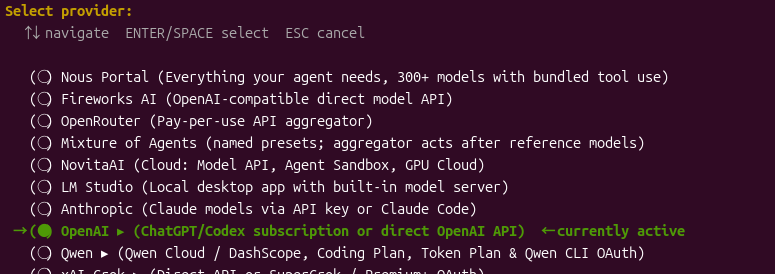
\includegraphics[width=0.85\linewidth]{docs/figures/menu-openai.png}\par
{\footnotesize\color{muted} \cmd{hermes -p analyst model}의 provider 목록. 화살표 키로 \textbf{OpenAI}로 옮겨 \kbd{Enter}, 이어지는 메뉴에서 ChatGPT/Codex 구독과 모델을 고릅니다.}
\end{center}
\warn{PI에서는 \cmd{hermes model}로 ChatGPT를 고르지 않습니다}{\cmd{-p} 없이 \cmd{hermes model}에서 ChatGPT를 고르면 PI의 주 모델까지 ChatGPT로 바뀝니다. PI의 로그인은 위처럼 \cmd{auth add}로만 합니다.
\textbf{Nous Portal} 로그인을 권하는 화면이 나오면 \kbd{Ctrl}+\kbd{C}로 나옵니다. 별도 유료 서비스입니다.}

\subsubsection*{PI 대화 압축 요약도 ChatGPT로}
대화가 길어지면 Hermes가 앞부분을 요약해 줄입니다. PI는 이 요약을 로컬 모델 대신 ChatGPT에 맡깁니다 (긴 글 요약은 큰 모델이 더 정확합니다).
위에서 이미 로그인했으므로 두 줄이면 됩니다. PI의 주 모델은 로컬 모델 그대로입니다.
\begin{sh}
hermes config set auxiliary.compression.provider openai-codex
hermes config set auxiliary.compression.model gpt-6.1-terra
\end{sh}

\subsection{확인}
주 모델과 예비 모델을 한 명씩 봅니다.
\begin{sh}
hermes -p coder fallback list       # Primary: qwen3.6-35b-a3b
hermes -p writer fallback list      # Primary: qwen3.6-35b-a3b
hermes -p scholar fallback list     # Primary: qwen3.6-35b-a3b
hermes -p analyst fallback list     # Primary: gpt-6.1-sol
hermes -p reviewer fallback list    # Primary: gpt-6.1-sol
\end{sh}
\ok{줄마다 \cmd{Primary}가 \texttt{\#} 뒤에 적은 모델이고, \cmd{1.}에 \cmd{claude-opus-5-5}이 보입니다.}

이제 다섯 명이 모두 모델에 닿는지 한 줄씩 확인합니다. coder·writer·scholar의 요청은 \ref{sec:pitest}절처럼 \cmd{/slots}의 \cmd{id_task}를 늘려야 합니다.
\begin{sh}
hermes -p coder chat -q "OK라고만 답해"
hermes -p analyst chat -q "OK라고만 답해"
hermes -p reviewer chat -q "OK라고만 답해"
hermes -p writer chat -q "OK라고만 답해"
hermes -p scholar chat -q "OK라고만 답해"
\end{sh}
\ok{줄마다 \cmd{OK}가 나옵니다.}

\tip{이 매뉴얼은 직원마다 한 줄씩 칩니다}{앞으로 나오는 설정도 모두 \cmd{-p <직원>}만 바꿔 한 명씩 실행합니다.
그래서 나중에 직원을 새로 늘려도 같은 줄을 그 이름으로 한 번 더 치면 됩니다 (\ref{sec:newmember}절 ``새 직원 추가하기'').}

% ================================================================
\chapter{다른 모델 고르기}
\label{sec:pickmodel}

4장의 구성(로컬 모델 4명 + ChatGPT 2명 + 예비 Claude Opus)은 기본값입니다. 직원별로 다른 모델을 쓰고 싶을 때 이 장을 봅니다.
처음 설치할 때는 건너뛰고 6장으로 가도 됩니다.

\section{바꿀 때마다 지키는 순서}
\begin{enumerate}[label=\textbf{\arabic*.}]
\item \textbf{단독 시험}: \cmd{hermes chat --provider <provider> -m <모델> -q "OK라고만 답해"}가 통과하는지 봅니다.
\item \textbf{바꾸기}: 아래 표의 명령을 실행합니다. \cmd{<직원>}은 \cmd{default}(PI), \cmd{coder}, \cmd{analyst}, \cmd{reviewer}, \cmd{writer}, \cmd{scholar} 중 하나입니다.
\item \textbf{적용}: \cmd{hermes gateway restart --all} 후, Discord에서 그 직원과 대화하던 채널에 \cmd{/reset}을 보냅니다 (열린 대화는 옛 모델을 붙잡고 있습니다).
\item \textbf{확인}: \cmd{hermes -p <직원> fallback list}에서 \cmd{Primary}와 예비 목록을 봅니다.
\end{enumerate}

\section{주 모델 바꾸기}
\label{sec:changemain}

\begin{center}
\small
\begin{longtable}{L{0.26\linewidth} L{0.66\linewidth}}
\toprule
\head \textbf{하고 싶은 것} & \textbf{명령} \\
\midrule
\endhead
ChatGPT의 다른 모델로 & \cmd{hermes -p <직원> model} → \textbf{OpenAI (ChatGPT/Codex subscription …)} → 목록에서 모델 선택 \\
로컬 모델 → ChatGPT로 & 메뉴: \cmd{hermes -p <직원> model} → \textbf{OpenAI (ChatGPT/Codex subscription …)} → 모델 선택\newline
  또는 명령 (로그인이 안 되어 있으면 먼저 \cmd{hermes auth add openai-codex}):\newline
  \cmd{hermes -p <직원> config set model.provider openai-codex}\newline
  \cmd{hermes -p <직원> config set model.default gpt-6.1-sol} \\
ChatGPT → 로컬 모델로\newline(예: analyst도 로컬) & \cmd{hermes -p <직원> config set model.provider custom:local-qwen}\newline
  \cmd{hermes -p <직원> config set model.default qwen3.6-35b-a3b}\newline
  (주소·문맥 길이는 복제 때 이미 들어 있습니다) \\
다른 로컬 모델로\newline(서버에 다른 모델을 띄웠을 때) & 새 모델의 \cmd{--alias}가 \cmd{<이름>}이면:\newline
  \cmd{hermes -p <직원> config set model.default <이름>}\newline
  \cmd{hermes -p <직원> config set providers.local-qwen.default_model <이름>}\newline
  문맥 길이가 다르면 \cmd{model.context_length}도 슬롯당 길이로 \\
로컬 모델 포트가 바뀌었을 때 & \cmd{hermes -p <직원> config set providers.local-qwen.base_url http://127.0.0.1:<새포트>/v1} \\
처음 상태로 & \cmd{.before-local} 백업을 덮어씁니다 (\ref{sec:tolocal}절 팁) \\
\bottomrule
\end{longtable}
\end{center}

\tip{GPU 없이 먼저 시작하고 싶다면}{로컬 모델 서버가 아직 없거나 점검 중이면, 4명을 ``로컬 모델 → ChatGPT로'' 명령으로 바꿔 6명 모두 ChatGPT로 돌릴 수 있습니다.
ChatGPT 사용량이 그만큼 늘어 한도에 더 자주 걸립니다. 서버가 준비되면 ``ChatGPT → 로컬 모델로''로 되돌립니다.}

\section{예비 모델 바꾸기}
\ref{sec:fallback}절의 \cmd{FB='...'} 줄만 아래 중 하나로 바꿔 실행하고, 이어서 바꿀 직원마다
\cmd{hermes -p <직원> config set fallback_providers "$FB"}를 한 줄씩 실행합니다.

\begin{center}
\small
\begin{longtable}{L{0.22\linewidth} L{0.7\linewidth}}
\toprule
\head \textbf{선택} & \textbf{FB 값과 특징} \\
\midrule
\endhead
Claude Opus\newline(기본) &
  \cmd{FB='[{"provider": "claude-subscription-directsdk-experimental", "model": "claude-opus-5-5", "base_url": "process://claude-subscription-directsdk-experimental", "api_mode": "chat_completions"}]'}\newline
  가장 똑똑하고 문맥이 깁니다. Claude 사용량을 많이 씁니다 \\
\midrule
Claude Sonnet &
  \cmd{FB='[{"provider": "claude-subscription-directsdk-experimental", "model": "claude-sonnet-5-5", "base_url": "process://claude-subscription-directsdk-experimental", "api_mode": "chat_completions"}]'}\newline
  더 빠르고 사용량을 덜 씁니다. Claude Code와 사용량을 나눠 쓰는 것이 걱정될 때 \\
\midrule
ChatGPT &
  \cmd{FB='[{"provider": "openai-codex", "model": "gpt-6.1-sol"}]'}\newline
  로컬 모델 직원 4명에게만 의미가 있습니다. analyst·reviewer는 주 모델과 같은 계정이라, 한도에 걸리면 예비도 같이 막힙니다 \\
\midrule
두 단계\newline(Claude → ChatGPT) &
  \cmd{FB='[{"provider": "claude-subscription-directsdk-experimental", "model": "claude-opus-5-5", "base_url": "process://claude-subscription-directsdk-experimental", "api_mode": "chat_completions"}, {"provider": "openai-codex", "model": "gpt-6.1-sol"}]'}\newline
  목록 순서대로 시도합니다. Claude까지 실패하면 ChatGPT \\
\midrule
예비 없음 &
  \cmd{FB='[]'}\newline
  ChatGPT 한도에 걸린 kanban 카드는 실패로 세지 않고 기다렸다가 한도가 풀리면 다시 시작합니다.
  대신 로컬 모델 서버가 꺼지면 4명의 일이 실패하고, 2번 실패한 kanban 카드는 \cmd{blocked}가 됩니다 \\
\bottomrule
\end{longtable}
\end{center}

\tip{메뉴로 고르고 싶다면}{\cmd{hermes -p <직원> fallback add}는 \cmd{hermes model}과 같은 메뉴로 예비 모델을 목록 끝에 하나 추가합니다. Claude는 \textbf{Claude Subscription DirectSDK (Experimental)}을 고릅니다 (\ref{sec:fallback}절 그림).
\cmd{fallback remove}는 하나를 골라 지우고, \cmd{fallback clear}는 모두 지웁니다 (\cmd{y}로 확인).}

\section{그 밖에 바꿀 수 있는 것}
\begin{center}
\small
\begin{tabular}{L{0.24\linewidth} L{0.68\linewidth}}
\toprule
\head \textbf{무엇} & \textbf{방법} \\
\midrule
PI 대화 압축 요약 모델 & \cmd{hermes config set auxiliary.compression.model <모델>} (ChatGPT 모델 이름) \\
생각 깊이 (reasoning) & \cmd{team.json}의 \cmd{"reasoning"}에서 직원별 \cmd{low}/\cmd{medium}/\cmd{high}를 고친 뒤 \cmd{python3 tools/lab.py reasoning} \\
지금 설정 보기 & \cmd{hermes -p <직원> config get model.default}, \cmd{hermes -p <직원> fallback list} \\
\bottomrule
\end{tabular}
\end{center}


% ================================================================
\chapter{팀으로 묶기}

지금은 직원 6명이 각자 따로 있습니다. 이 장에서 서로 멘션하며 협업하고, 역할 규칙을 지키고, 프로젝트 채널을 다룰 수 있게 묶습니다.
대부분은 설치 도우미 스크립트가 해 주므로 \textbf{ID만 정확히 적으면} 됩니다.

\section{팀 설정 파일 채우기}
\does{기록표의 ID를 두 파일에 옮겨 적습니다. 이후 모든 스크립트가 이 값을 읽습니다.}

\subsection{team.json}
\begin{sh}
cd ~/Projects/hermes-team
nano team.json
\end{sh}
\cmd{guild_id}, \cmd{category_id}, \cmd{lobby_channels} 세 곳의 숫자를 기록표 값으로 바꿉니다. 나머지는 그대로 둡니다.
\begin{filebox}{~/Projects/hermes-team/team.json (예)}
\begin{code}
{
  "guild_id": "111111111111111111",          ← 서버(guild) ID
  "category_id": "222222222222222222",       ← Projects 카테고리 ID
  "projects_root": "~/Projects",
  "profiles": ["default", "coder", "analyst", "reviewer", "writer", "scholar"],
  "lobby_channels": ["333333333333333333"],  ← 로비 채널(#hermes) ID
  "reasoning": {
    "default": "medium", "coder": "low", "analyst": "medium",
    "reviewer": "medium", "writer": "low", "scholar": "low"
  }
}
\end{code}
\end{filebox}
\warn{화살표와 설명은 적지 않습니다}{위 예의 \cmd{← ...}는 설명입니다. 실제 파일에 넣으면 JSON이 깨집니다.
숫자는 따옴표 \cmd{" "} 안에 넣고, 쉼표와 괄호는 그대로 둡니다.}

\subsection{souls/\_team\_ids.md}
\begin{sh}
nano souls/_team_ids.md
\end{sh}
맨 위 일곱 줄의 대문자 자리(\cmd{RESEARCHER_USER_ID}, \cmd{PI_BOT_ID} …)를 기록표의 \textbf{내 사용자 ID}와 \textbf{봇 ID}로 바꿉니다.
\cmd{<@ >} 기호는 그대로 둡니다. 연구자 이름 자리는 \cmd{set_name.sh}가 이미 채웠습니다.
\begin{filebox}{~/Projects/hermes-team/souls/\_team\_ids.md (위쪽)}
\begin{code}
## 팀 Discord ID (멘션할 때 이 형식을 그대로 쓴다)
- 연구자 minji: `<@444444444444444444>`
- PI: `<@555555555555555555>`
- coder: `<@666666666666666666>`
- analyst: `<@777777777777777777>`
- reviewer: `<@888888888888888888>`
- writer: `<@999999999999999999>`
- scholar: `<@000000000000000000>`
\end{code}
\end{filebox}
\tip{Application ID가 아니라 봇 ID}{여기에는 4.1절 5번에서 멤버 목록을 우클릭해 복사한 \textbf{봇 ID}를 넣습니다.}

\section{게이트웨이를 서비스로 켜기}
\label{sec:gwservice}
\does{직원 6명을 한꺼번에 맡는 게이트웨이를 systemd 서비스로 등록하고 켭니다. 이후의 \cmd{restart}는 모두 이 서비스를 다시 시작합니다.}
혹시 \cmd{hermes gateway run}으로 띄워 둔 게이트웨이가 있으면 먼저 끕니다(그 창에서 \kbd{Ctrl}+\kbd{C}). 같은 봇이 두 번 뜨면 나중에 켠 쪽이 연결에 실패합니다.
\begin{sh}
hermes gateway install
hermes gateway status
\end{sh}
질문 두 개(\cmd{Start the gateway now ...?}, \cmd{... automatically on login/boot with systemd?})에는 둘 다 \cmd{y}.
\begin{out}
● hermes-gateway.service - Hermes Agent gateway
     Active: active (running) since ...
\end{out}
\ok{\cmd{hermes-gateway.service}와 \cmd{active (running)}이 보입니다. Discord 멤버 목록에서 봇 6개가 온라인(초록 점)이 됩니다.}
\warn{\cmd{Failed to enable unit: ... does not exist}가 나오면}{gnode1이 내 홈을 아직 \cmd{/home/<계정>}으로 보고 있는 것입니다. \ref{sec:gwfix}절을 따릅니다.}

\section{한 번에 적용하기}
\does{위 두 파일을 읽어 6명의 협업 설정, 생각 깊이, 채널 연결, 역할 규칙(SOUL)을 한꺼번에 설치합니다.}
\begin{sh}
cd ~/Projects/hermes-team
python3 tools/lab.py env         # 6명 .env: 봇끼리 멘션 허용, 허용 사용자 = 나 + 봇 6개
python3 tools/lab.py reasoning   # 생각 깊이: PI·analyst·reviewer medium / coder·writer·scholar low
python3 newproject.py sync       # 6명 config.yaml: 로비·프로젝트 채널 연결 (PI만 멘션 없이 응답)
bash install_souls.sh            # 6명 SOUL(역할·규칙) 설치 + 게이트웨이 재시작
\end{sh}

\begin{itemize}
\item \cmd{lab.py env}는 각 직원의 \cmd{.env}에 협업 설정(\cmd{DISCORD_ALLOW_BOTS=mentions} 등)과 허용 사용자 7명을 적습니다. 원본은 \cmd{.env.bak}으로 남습니다.
\item \cmd{install_souls.sh}가 \textbf{``주의: 채우지 않은 ID''}를 출력하면 6.1절로 돌아가 빠진 ID를 채우고 다시 실행합니다.
\end{itemize}
\ok{네 명령이 오류 없이 끝나고, \cmd{install_souls.sh}가 ID 경고 없이 게이트웨이를 재시작합니다.}
\warn{게이트웨이가 이 창을 차지하면 (\cmd{Press Ctrl+C to stop})}{게이트웨이가 서비스로 등록되지 않은 것입니다(\ref{sec:gwservice}절). \kbd{Ctrl}+\kbd{C}로 끄고 \ref{sec:gwservice}절부터 다시 합니다. 등록이 실패하면 \ref{sec:gwfix}절을 봅니다.}

\section{직원 봇의 슬래시 명령 등록 (처음 한 번)}
\label{sec:sync}
\does{\cmd{/reset} 같은 Discord 명령을 직원 봇 5개에도 등록합니다.}

복제한 profile은 PI의 ``명령 등록 완료'' 기록까지 복사돼서, 그대로 두면 직원 봇에 명령이 생기지 않습니다. 한 번만 강제로 등록합니다.
아래를 붙여 넣습니다 (마지막에 30초 기다립니다).
\begin{sh}
echo 'DISCORD_COMMAND_SYNC_POLICY=bulk' >> ~/.hermes/profiles/coder/.env
echo 'DISCORD_COMMAND_SYNC_POLICY=bulk' >> ~/.hermes/profiles/analyst/.env
echo 'DISCORD_COMMAND_SYNC_POLICY=bulk' >> ~/.hermes/profiles/reviewer/.env
echo 'DISCORD_COMMAND_SYNC_POLICY=bulk' >> ~/.hermes/profiles/writer/.env
echo 'DISCORD_COMMAND_SYNC_POLICY=bulk' >> ~/.hermes/profiles/scholar/.env
hermes gateway restart --all
sleep 30
\end{sh}
직원마다 등록 기록이 생겼는지 한 줄씩 봅니다. 숫자는 등록한 횟수입니다.
\begin{sh}
grep -c -i 'Synced.*slash' ~/.hermes/profiles/coder/logs/gateway.log
grep -c -i 'Synced.*slash' ~/.hermes/profiles/analyst/logs/gateway.log
grep -c -i 'Synced.*slash' ~/.hermes/profiles/reviewer/logs/gateway.log
grep -c -i 'Synced.*slash' ~/.hermes/profiles/writer/logs/gateway.log
grep -c -i 'Synced.*slash' ~/.hermes/profiles/scholar/logs/gateway.log
\end{sh}
\ok{다섯 줄 모두 \cmd{1} 이상입니다.}
\warn{\cmd{0}인 직원이 있으면}{30초로 모자랐을 수 있습니다. 1분쯤 더 기다렸다가 그 줄만 다시 실행합니다. 그래도 \cmd{0}이면 그 직원의 \cmd{.env}에 강제 등록 줄이 들어갔는지(\cmd{grep SYNC ~/.hermes/profiles/<직원>/.env}) 보고, \cmd{hermes gateway restart --all} 후 다시 확인합니다.}
등록이 끝났으니 강제 등록 줄을 다시 지웁니다. 남겨 두면 재시작할 때마다 명령을 새로 등록합니다.
\begin{sh}
sed -i '/^DISCORD_COMMAND_SYNC_POLICY=bulk$/d' ~/.hermes/profiles/coder/.env
sed -i '/^DISCORD_COMMAND_SYNC_POLICY=bulk$/d' ~/.hermes/profiles/analyst/.env
sed -i '/^DISCORD_COMMAND_SYNC_POLICY=bulk$/d' ~/.hermes/profiles/reviewer/.env
sed -i '/^DISCORD_COMMAND_SYNC_POLICY=bulk$/d' ~/.hermes/profiles/writer/.env
sed -i '/^DISCORD_COMMAND_SYNC_POLICY=bulk$/d' ~/.hermes/profiles/scholar/.env
hermes gateway restart --all
\end{sh}
\ok{Discord에서 \kbd{Ctrl}+\kbd{R}로 새로고침하고 채팅창에 \cmd{/}를 입력하면 봇마다 명령 목록이 보입니다.}

\section{PI에게 채널 만들 권한 주기}
\does{PI가 새 프로젝트 채널을 \cmd{Projects} 카테고리 안에 만들 수 있게 합니다.}

Discord에서 \cmd{Projects} 카테고리 이름 우클릭 → \textbf{카테고리 편집} → \textbf{권한} → \textbf{멤버 또는 역할 추가} → \cmd{hermes-researcher} →
\textbf{채널 관리}를 초록 체크(허용)로 → \textbf{변경 사항 저장}.

\tip{서버 전체가 아니라 카테고리에만}{서버 전체 관리 권한을 주지 않고 이 카테고리 안에서만 허용하는 것이 안전합니다.}

\section{Antigravity 읽기 권한}
\does{scholar가 학술 사이트를 읽을 수 있게 허용하고, 페이지 조작은 막습니다.}

\cmd{agy -p} 같은 무인 실행은 허용되지 않은 사이트 읽기를 \textbf{오류 없이 조용히 거부}합니다. 그래서 미리 허용 목록을 넣어 둡니다.
\begin{sh}
python3 ~/Projects/hermes-team/tools/lab.py agy-perms
\end{sh}
학술 도메인 20개 읽기 허용과 페이지 조작 거부 규칙이 \cmd{~/.gemini/antigravity-cli/settings.json}에 합쳐집니다. 기존 규칙은 유지되고 원본은 \cmd{settings.json.bak}으로 남습니다.

\section{자동 장치 설치 (아침 브리핑, 차단 감시, PI 인계)}
\does{사람이 챙기지 않아도 돌아가는 자동 장치 세 가지를 설치합니다.}

\begin{center}
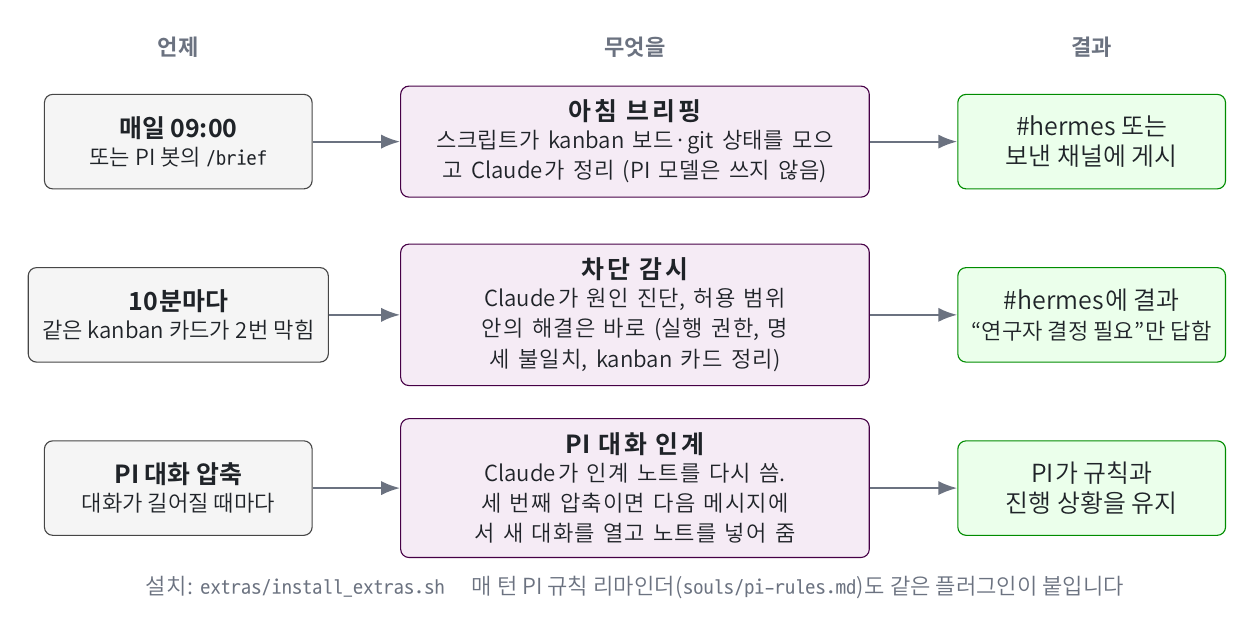
\includegraphics[width=\linewidth]{docs/figures/auto.png}
\end{center}

\begin{center}
\small
\begin{tabular}{L{0.2\linewidth} L{0.7\linewidth}}
\toprule
\head \textbf{장치} & \textbf{하는 일} \\
\midrule
아침 브리핑 & 매일 09:00 프로젝트 상태를 Claude가 정리해 \ch{hermes}에 올립니다. Discord에서 PI 봇의 \cmd{/brief}로 언제든 받을 수도 있습니다 \\
차단 감시 & 10분마다 확인해, 같은 일이 2번 이상 막히면 Claude가 원인을 진단하고 허용 범위 안에서 바로 고친 뒤 \ch{hermes}로 알립니다 \\
PI 대화 인계 & PI 대화가 길어지면 규칙을 놓치므로, 인계 노트를 써 두었다가 새 대화를 열 때 자동으로 넣어 줍니다 \\
\bottomrule
\end{tabular}
\end{center}

\begin{sh}
bash ~/Projects/hermes-team/extras/install_extras.sh
bash ~/Projects/hermes-team/install_souls.sh      # 게이트웨이 재시작 → hook·플러그인 적용
hermes plugins list | grep lab-handoff
hermes cron status
hermes cron list
\end{sh}
\ok{\cmd{lab-handoff}가 \cmd{enabled}이고, \cmd{hermes cron status}에 \cmd{Gateway is running}과 \cmd{2 active job(s)}가 보입니다.
\cmd{hermes cron list}에서 \cmd{morning-brief}의 \cmd{Next run}이 \textbf{다음 09:00 (+09:00)}입니다.}
\tip{\cmd{cron status}의 Next run이 10분 안쪽이면}{정상입니다. 두 작업 중 가장 가까운 것을 보여 주는데, 차단 감시가 10분마다 돌기 때문입니다.}

\warn{브리핑 시각이 9시간 어긋나면}{서버 시간대가 UTC인 경우입니다 (\cmd{date}로 확인). 공용 서버의 시간대는 바꾸지 말고,
브리핑 cron을 UTC 기준 \cmd{"0 0 * * *"}(한국 시각 09:00)로 다시 만듭니다.}

\tip{여러 번 실행해도 됩니다}{\cmd{install_extras.sh}는 이미 있는 것은 건너뜁니다. \cmd{extras/}의 파일을 고친 뒤에도 다시 실행합니다.}

\section{PI 홈 채널 정하기}
\does{PI가 브리핑과 알림을 보낼 기본 채널을 \ch{hermes}로 정합니다.}

Discord \ch{hermes} 채널에서 \cmd{/sethome}을 입력합니다. 봇 6개가 모두 같은 명령을 갖고 있어서 목록에 \cmd{/sethome}이 여러 줄 뜹니다.
아이콘이 모두 같으므로 \textbf{오른쪽 끝의 봇 이름}을 보고, \textbf{hermes-researcher}(PI) 줄을 골라 보냅니다.
\begin{center}
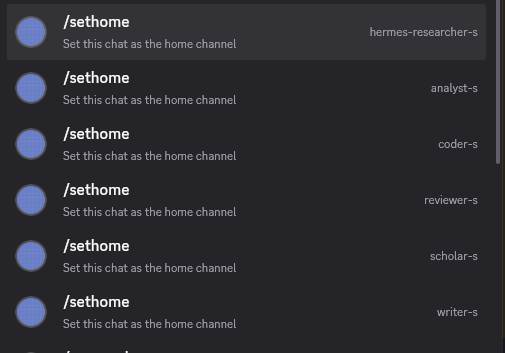
\includegraphics[width=0.62\linewidth]{docs/figures/discord-sethome.png}\par
{\footnotesize\color{muted} 맨 위 줄처럼 오른쪽에 \textbf{hermes-researcher}가 적힌 항목을 고릅니다. 다른 줄을 고르면 그 직원의 홈 채널이 바뀝니다.}
\end{center}
\tip{봇마다 아이콘을 달아 두면 헷갈리지 않습니다}{Discord 개발자 페이지(4.1절)에서 봇을 고른 뒤 두 곳에 그림을 올립니다.
\textbf{General Information} → \textbf{App Icon}은 위 그림 같은 \textbf{명령 목록}의 아이콘, \textbf{Bot} → \textbf{Icon}은 \textbf{멤버 목록과 대화}에 보이는 봇 프로필 사진입니다.
\textbf{Save Changes}를 누르면 바로 바뀌고, 서버에 다시 초대할 필요는 없습니다. 안 바뀌어 보이면 Discord 앱에서 \kbd{Ctrl}+\kbd{R}로 새로고침합니다.}

이어서 터미널에서 브리핑을 한 번 시험합니다.
\begin{sh}
hermes cron run morning-brief
\end{sh}
\ok{1\textasciitilde3분 뒤 \ch{hermes}에 브리핑이 올라옵니다 (아직 프로젝트가 없으므로 내용은 짧습니다).}

\section{SSH를 끊어도 계속 도는지 확인}
\label{sec:linger}
\does{로그인하지 않아도, 서버를 다시 켜도 게이트웨이가 저절로 도는지 확인합니다.}
\begin{sh}
loginctl show-user $USER -p Linger
hermes gateway status
\end{sh}
linger는 ``내가 SSH 접속을 끊어도 내 서비스를 계속 돌려라''라는 설정입니다. 이게 없으면 SSH를 끊는 순간 직원들도 같이 꺼집니다.
\begin{out}
Linger=yes
● hermes-gateway.service - Hermes Agent gateway
     Active: active (running) since Thu 2026-11-06 14:02:11 KST; 3h ago
\end{out}
\ok{\cmd{Linger=yes}이고 \cmd{active (running)}이면 SSH를 끊어도, 서버를 다시 켜도 직원들이 계속 일합니다.}
\tip{확실히 해 보려면}{SSH를 끊었다가 다시 접속해 \cmd{hermes gateway status}를 봅니다. \cmd{since} 시각이 그대로면 그동안 한 번도 꺼지지 않은 것입니다.
게이트웨이를 끄고 켤 때는 \cmd{hermes gateway stop} / \cmd{hermes gateway start}를 씁니다.}

\subsection{서비스가 등록되지 않을 때 (홈 경로 문제)}
\label{sec:gwfix}
\cmd{hermes gateway install}이 아래처럼 \cmd{Failed to enable unit: ... does not exist}로 끝나면, systemd가 내 홈을 \cmd{/home/<계정>}으로 보고 있는 것입니다(\ref{sec:svchome}절의 확인이 통과하지 않은 경우).
서비스 파일은 \cmd{/ai/works/<계정>/.config/systemd/user/}에 만들어졌는데, systemd는 \cmd{/home/<계정>} 쪽에서 찾기 때문입니다.
\begin{center}
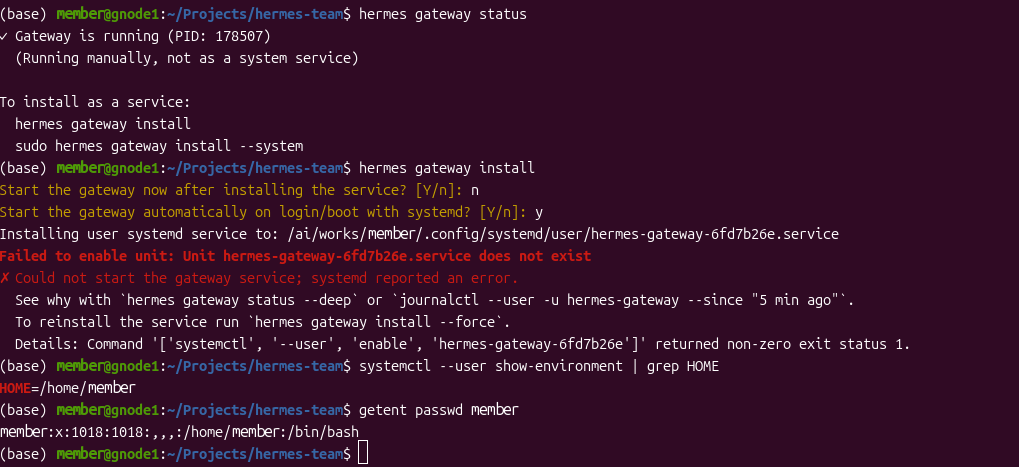
\includegraphics[width=\linewidth]{docs/figures/gateway-install-fail.png}\par
{\footnotesize\color{muted} gnode1에서 실제로 나온 화면. 아래 두 줄이 \cmd{/home/<계정>}을 가리키는 것이 원인입니다.}
\end{center}

\textbf{① 원인 확인.} 아래 두 줄이 모두 \cmd{/home/<계정>}을 보여 주면 이 문제입니다.
\begin{sh}
systemctl --user show-environment | grep HOME
getent passwd $USER
\end{sh}

\textbf{② 관리자에게 부탁.} 위 화면을 캡처해 보내며 이렇게 부탁합니다. 계정을 새로 만드는 것이 아니라, \textbf{같은 UID 그대로 gnode1에서만 홈 경로를 바꾸는} 것입니다.
\begin{msg}[관리자에게 보낼 메시지]
gnode1에서 systemd 사용자 서비스가 제 홈을 /home/<계정>으로 보고 있어 서비스 등록이 안 됩니다(캡처 첨부).
gnode1의 \texttt{/etc/passwd}에 아래 한 줄을 추가해 주실 수 있을까요? UID·GID는 \texttt{getent passwd <계정>} 결과와 같고 홈만 다릅니다.\par\smallskip
\texttt{<계정>:x:<UID>:<GID>:,,,:/ai/works/<계정>:/bin/bash}\par\smallskip
nsswitch.conf가 files를 NIS보다 먼저 보므로 다른 노드에는 영향이 없습니다.
추가 후 \texttt{systemctl restart user@<UID>}도 부탁드립니다. (Linger가 no라면 \texttt{loginctl enable-linger <계정>}도 함께)
\end{msg}

\textbf{③ 고쳐질 때까지는 6장을 멈춥니다.} 게이트웨이는 서비스로 등록한 뒤에 켭니다. 관리자가 설정해 주면 아래 ④부터 이어서 합니다.

\textbf{④ 관리자가 고쳐 준 뒤: 사용자 systemd 다시 띄우기.} 먼저 계정 정보가 바뀌었는지 봅니다.
\begin{sh}
getent passwd $USER
\end{sh}
\ok{\cmd{/ai/works/<계정>}이 보입니다. 아직 \cmd{/home/<계정>}이면 관리자 설정이 반영되지 않은 것이니 관리자에게 다시 확인합니다.}
여기서 끝이 아닙니다. 내 사용자 systemd는 \textbf{예전 홈일 때 시작되어 그때 정한 경로에서만 서비스 파일을 찾고} 있고,
Linger가 켜져 있어 SSH를 끊어도 꺼지지 않습니다. \cmd{show-environment}의 \cmd{HOME}이 새 값으로 보여도, \cmd{daemon-reload}를 해도 찾는 경로는 그대로입니다.
그래서 systemd를 한 번 내렸다가 새로 띄웁니다. sudo는 필요 없습니다.
\begin{sh}
systemctl --user exit
\end{sh}
그다음 \textbf{SSH를 모두 끊고 다시 접속}해서, systemd가 실제로 찾는 경로(\cmd{UnitPath})에 새 홈이 들어갔는지 확인합니다.
\begin{sh}
systemctl --user show -p UnitPath | tr ' ' '\n' | grep works
\end{sh}
\begin{out}
/ai/works/minji/.config/systemd/user.control
/ai/works/minji/.config/systemd/user
...
\end{out}
\ok{\cmd{/ai/works/<계정>/.config/systemd/user}가 보입니다.
아무것도 안 나오면 관리자에게 \cmd{sudo systemctl restart user@<UID>}를 부탁합니다.}
\tip{\cmd{systemd-analyze --user unit-paths}로 확인하면 안 됩니다}{이 명령은 systemd에 묻지 않고 \textbf{지금 셸의 HOME}으로 경로를 계산하므로, systemd가 예전 경로를 보고 있어도 정상처럼 나옵니다. 꼭 \cmd{systemctl --user show -p UnitPath}로 봅니다.}

\textbf{⑤ 서비스로 등록.} 먼저 정리합니다.
\begin{itemize}
\item \cmd{hermes gateway run}으로 켜 둔 창이 있으면 \kbd{Ctrl}+\kbd{C}로 끕니다. 같은 봇이 두 번 뜨지 않도록 \textbf{먼저 끄는 것}이 중요합니다.
\item 실패할 때 남은 예전 서비스 파일(\cmd{hermes-gateway-}\textit{숫자·영문}\cmd{.service})이 있으면 지웁니다. 남겨 두면 나중에 게이트웨이가 두 개 뜰 수 있습니다.
\end{itemize}
\begin{sh}
ls ~/.config/systemd/user/
rm -f ~/.config/systemd/user/hermes-gateway-*.service
\end{sh}
이제 등록합니다. 질문 두 개(\cmd{Start the gateway now ...?}, \cmd{... automatically on login/boot ...?})에는 둘 다 \cmd{y}.
\begin{sh}
hermes gateway install --force
hermes gateway status
python3 ~/Projects/hermes-team/tools/lab.py check
\end{sh}
\ok{\cmd{hermes gateway status}에 \cmd{hermes-gateway.service}와 \cmd{active (running)}이 보이고, \cmd{lab.py check}의 게이트웨이 줄이 OK입니다.
이제 SSH를 끊어도, 서버를 다시 켜도 직원들이 계속 일합니다. 끄고 켤 때는 \cmd{hermes gateway stop} / \cmd{start}를 씁니다.
6장을 진행하던 중이었다면 \ref{sec:gwservice}절 다음부터 이어서 합니다.}

% ================================================================
\chapter{점검과 첫 대화}

\section{자동 점검}
\does{지금까지의 설치를 한 번에 확인합니다. 아무것도 바꾸지 않으니 언제 실행해도 안전합니다.}
\begin{sh}
python3 ~/Projects/hermes-team/tools/lab.py check
\end{sh}
도구, 팀 설정, 6명의 토큰 중복 여부, 협업 설정, SOUL 최신 여부, 채널 연결, 생각 깊이, 게이트웨이, 아침 브리핑, Antigravity 권한을 차례로 봅니다.
\begin{out}
OK     hermes v0.22.5
OK     team.json: guild / category / lobby
...
READY — 모든 점검 통과
\end{out}
\ok{마지막 줄이 \cmd{READY}입니다.}

\cmd{WARN} 줄이 있으면 그 줄에 고치는 명령이 함께 나옵니다. 그 명령을 실행하고 \cmd{check}를 다시 돌립니다.

\section{Discord에서 시험하기}
\label{sec:firsttest}
아래를 위에서부터 차례로 해 봅니다.

\begin{center}
\small
\begin{longtable}{c L{0.15\linewidth} L{0.3\linewidth} L{0.42\linewidth}}
\toprule
\head \textbf{\#} & \textbf{어디서} & \textbf{보낼 메시지} & \textbf{기대 결과} \\
\midrule
\endhead
1 & \ch{hermes} & \cmd{넌 누구야?} (멘션 없이) & PI만 답합니다 \\
2 & \ch{hermes} & \cmd{@coder 넌 누구야?} & coder만 답합니다. PI는 \cmd{—}만 보내거나 조용합니다 \\
3 & \ch{hermes} & analyst, reviewer, writer, scholar에게도 2번처럼 & 각자 자기 역할을 소개합니다 \\
4 & \ch{hermes} & \cmd{새 프로젝트 만들자: 간단한 선형회귀} & PI가 이름·태그를 제안 → \cmd{승인} → \cmd{Projects}에 새 채널, \cmd{~/Projects/<이름>} 폴더, kanban 보드가 생기고 링크를 보고합니다.
  \textbf{보고 직후 게이트웨이가 15초 뒤 재시작됩니다} \\
5 & 새 프로젝트 채널 (\textbf{30초쯤 기다렸다가}) & \cmd{상태 알려줘} & 첫 줄에 \cmd{[태그]}, 표 형식 상태 보고. PI는 새 채널에서 먼저 말을 걸지 않으므로 내가 첫 메시지를 보냅니다 \\
6 & 새 프로젝트 채널 & \cmd{데이터 생성 스크립트 하나 만들어줘} & PI가 kanban 카드 생성 → coder가 Claude Code로 작성 → reviewer 검토 → PI가 \cmd{main}에 commit \\
7 & 새 프로젝트 채널 & \cmd{@coder 기억해: 코드 스타일 — 타입 힌트 필수} & 답 끝에 \cmd{기억함: ...} \\
\bottomrule
\end{longtable}
\end{center}

\tip{멘션하는 법}{\cmd{@}를 입력하고 자동완성 목록에서 \textbf{APP} 표시가 붙은 봇을 고릅니다. 같은 이름의 \emph{역할(role)}을 고르면 봇이 반응하지 않습니다.}

4번을 실제로 해 본 화면입니다. PI가 이름·태그·설명을 제안하면 \cmd{승인}(또는 \cmd{좋아})으로 답하고, 바꾸고 싶으면 \cmd{이름은 lr-demo로} 처럼 고쳐 말합니다.
\begin{center}
\begin{minipage}[t]{0.41\linewidth}\centering
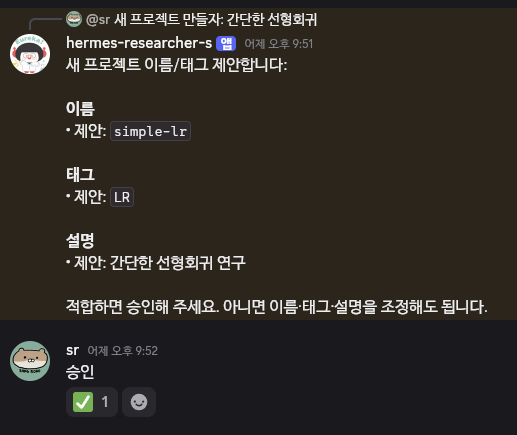
\includegraphics[width=\linewidth]{docs/figures/discord-newproject-1.png}\par\smallskip
{\footnotesize\color{muted} ① 요청 → PI의 제안 → \cmd{승인}}
\end{minipage}\hfill
\begin{minipage}[t]{0.41\linewidth}\centering
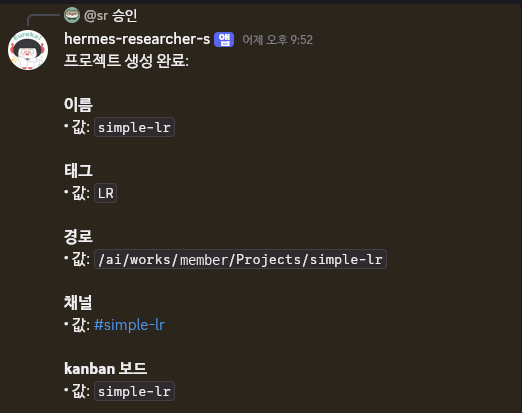
\includegraphics[width=\linewidth]{docs/figures/discord-newproject-2.png}\par\smallskip
{\footnotesize\color{muted} ② 생성 완료 보고 (경로·채널·kanban 보드)}
\end{minipage}\hfill
\begin{minipage}[t]{0.15\linewidth}\centering
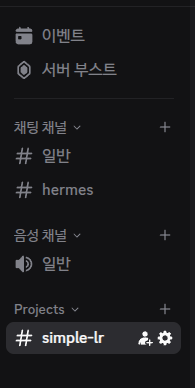
\includegraphics[width=\linewidth]{docs/figures/discord-newproject-3.png}\par\smallskip
{\footnotesize\color{muted} ③ \cmd{Projects}에 생긴 채널}
\end{minipage}
\end{center}
보고가 끝나고 15초쯤 뒤 게이트웨이가 다시 시작되며 봇들이 잠깐 오프라인이 됩니다. 30초쯤 기다렸다가 새 채널(여기서는 \ch{simple-lr})에서 5번을 보냅니다.

6번의 진행 상황은 터미널에서도 볼 수 있습니다.
\begin{sh}
hermes kanban --board <프로젝트> list
\end{sh}

\section{반응이 없을 때}
\begin{enumerate}
\item \textbf{재시작 중일 수 있습니다.} 30초\textasciitilde1분 기다렸다가 다시 보냅니다. 확인: \cmd{hermes gateway status}
\item 그래도 조용하면 그 채널에서 그 봇에게 \cmd{/reset}을 보냅니다 (\cmd{/} 입력 → 그 봇의 명령 목록에서 \cmd{/reset}). 이전 대화가 옛 설정을 붙잡고 있을 때 생깁니다.
\item 그래도 안 되면 채널이 등록됐는지 확인하고 게이트웨이를 다시 켭니다.
\end{enumerate}
\begin{sh}
python3 ~/Projects/hermes-team/newproject.py list
python3 ~/Projects/hermes-team/tools/lab.py check
hermes gateway restart --all
\end{sh}

\begin{center}
\begin{tcolorbox}[enhanced,colback=tipbg,colframe=tipc,boxrule=0.6pt,arc=4pt,width=0.8\linewidth,halign=center]
{\large\bfseries\color{tipc} 여기까지 왔다면 설치는 끝났습니다.}\par\smallskip
이제부터는 터미널 없이 Discord에서 일을 맡기면 됩니다. 다음 장은 매일 쓰는 법입니다.
\end{tcolorbox}
\end{center}

\section{예시: 분자 용해도 예측으로 연구 한 바퀴}
\label{sec:esol}
\does{\ch{simple-lr} 프로젝트에서 실제로 해 본 기록입니다. 아래 메시지를 같은 순서로 보내면 내 프로젝트에서도 가설 → 실험 → 결과 → 다음 단계를 한 바퀴 돌려 볼 수 있습니다.}

\textbf{주제.} 분자가 물에 얼마나 녹는지(\cmd{logS})를 분자 지표 4개로 선형회귀하는 고전 예제입니다.
Delaney(2004)가 ESOL이라는 이름으로 발표한 방법이고, 그 데이터(분자 1,128개)는 MoleculeNet의 \textbf{ESOL} 데이터셋으로 공개되어 있습니다.
지표 4개는 logP(기름/물 분배 계수), 분자량, 회전 가능한 결합 수, 방향족 비율(AROM)입니다. CPU로 몇 분이면 끝나서 GPU가 필요 없습니다.

\info{시작 전에}{새 프로젝트를 하나 만듭니다(\ref{sec:firsttest}절 4번처럼 \ch{hermes}에서 \cmd{새 프로젝트 만들자: 분자 용해도 선형회귀}). 아래 메시지는 모두 \textbf{그 프로젝트 채널}에 보냅니다.
gnode1에서 인터넷이 막혀 있으면 데이터 내려받기에서 멈춥니다. 그때는 ESOL CSV를 직접 받아 \cmd{~/Projects/<프로젝트>/data/}에 넣고 ``데이터는 \cmd{data/delaney.csv}에 있어''라고 알려 줍니다.}

\subsection*{① 가설 세우기}
\begin{msg}
ESOL 데이터로 분자 용해도(logS)를 선형회귀로 예측해 보려고 해. 가설: logP 하나만으로도 R²가 0.7 이상이고, 분자량·회전 결합 수·방향족 비율을 더하면 더 좋아진다. 가설로 정리해줘
\end{msg}
PI가 \cmd{HYPOTHESES.md}에 넣을 반영안(\cmd{H-001}, \cmd{H-002})을 가설·근거·검증 방법·지지/반증 기준으로 정리해 보여 줍니다. 아직 파일에 쓰지는 않았습니다.
\begin{center}
\begin{minipage}[t]{0.48\linewidth}\vspace{0pt}\centering
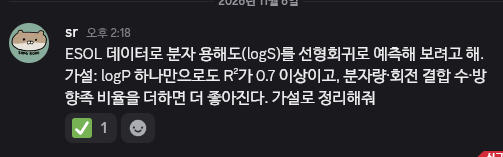
\includegraphics[width=\linewidth]{docs/figures/esol-1-ask.png}\par\smallskip{\footnotesize\color{muted} 내가 보낸 메시지}
\end{minipage}\hfill
\begin{minipage}[t]{0.48\linewidth}\vspace{0pt}\centering
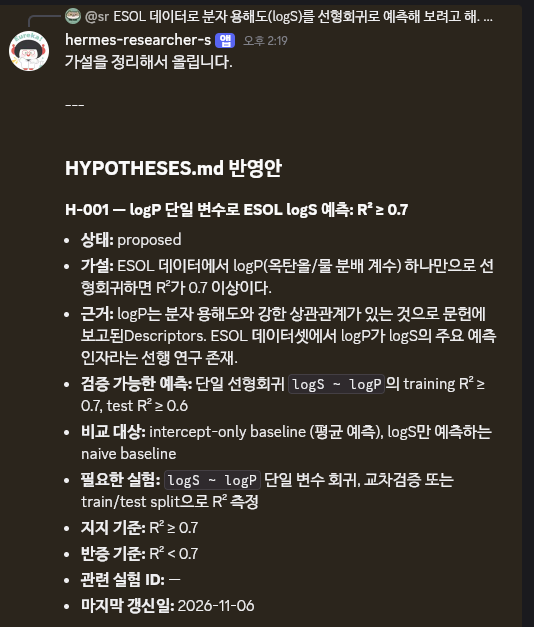
\includegraphics[width=\linewidth]{docs/figures/esol-2-hypothesis.png}\par\smallskip{\footnotesize\color{muted} PI의 가설 반영안 (H-001)}
\end{minipage}
\end{center}

\subsection*{② 직원의 질문에 답하고 승인}
반영안 끝에 \textbf{검토 사항}이 붙어 옵니다. 정의가 애매한 것(AROM을 어떻게 계산할지), 가설끼리의 관계, 변수를 더 넣을지처럼 \textbf{연구자가 정할 것}을 먼저 묻습니다.
무난하게 가려면 논문 정의를 그대로 쓰고 변수를 고정한다고 답한 뒤, 같은 메시지에서 승인합니다.
\begin{msg}
1. AROM은 Delaney 논문 정의대로 방향족 원자 수 / 무거운 원자(수소 제외) 수로 해. 데이터에 있는 열을 쓰지 말고 SMILES에서 RDKit으로 직접 계산해 (atom.GetIsAromatic() 개수 / mol.GetNumHeavyAtoms()). logP(Crippen.MolLogP), 분자량(Descriptors.MolWt), 회전 결합 수(Descriptors.NumRotatableBonds)도 RDKit으로 계산해.\par
2. 관계는 그렇게 이해한 게 맞아. H-001이 반증돼도 H-002는 그대로 돌리고, 결과만 같이 해석해.\par
3. 변수는 4개로 고정. HBD, PSA 같은 건 이번에는 넣지 마.\par\smallskip
이대로 가설 반영 승인. 다음은 실험 계획 세워줘.
\end{msg}
\begin{center}
\begin{minipage}[t]{0.48\linewidth}\vspace{0pt}\centering
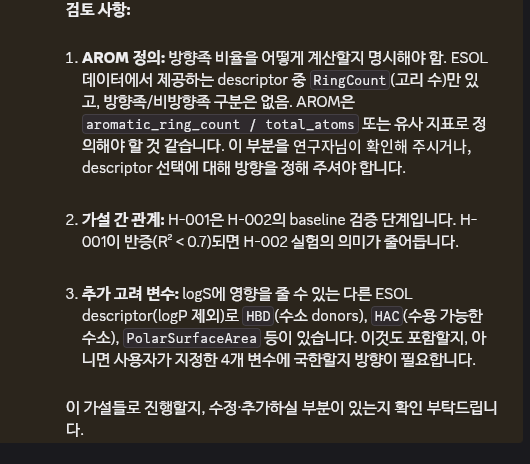
\includegraphics[width=\linewidth]{docs/figures/esol-3-review.png}\par\smallskip{\footnotesize\color{muted} PI의 검토 사항}
\end{minipage}\hfill
\begin{minipage}[t]{0.48\linewidth}\vspace{0pt}\centering
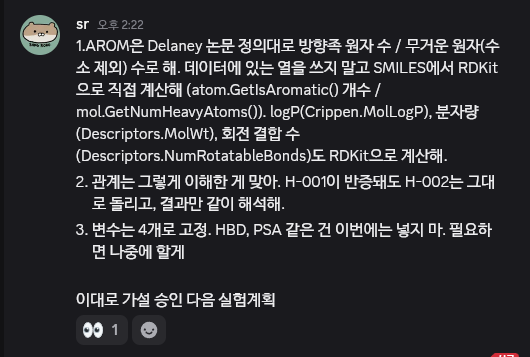
\includegraphics[width=\linewidth]{docs/figures/esol-4-answer.png}\par\smallskip{\footnotesize\color{muted} 내 답과 승인}
\end{minipage}
\end{center}

\subsection*{③ 패키지 설치 승인}
PI가 실험 명세와 코드를 준비해 commit한 뒤, 새 Python 패키지가 필요하면 \cmd{uv add} 승인을 묻습니다(\ref{sec:projtree}절의 승인 규칙).
\begin{msg}
승인
\end{msg}
\begin{center}
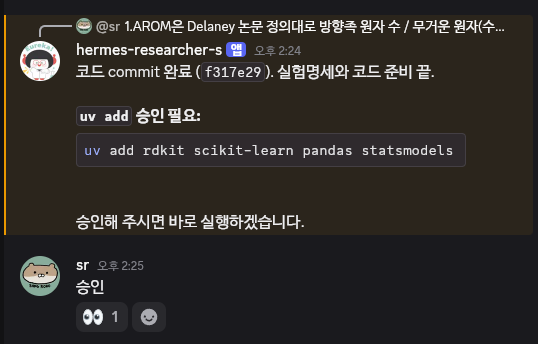
\includegraphics[width=0.55\linewidth]{docs/figures/esol-5-uvadd.png}\par\smallskip
{\footnotesize\color{muted} 코드 commit 후 \cmd{uv add} 승인 요청}
\end{center}

\subsection*{④ 결과 보고}
승인하면 바로 실행하고, 끝나면 가설별로 지지/반증과 수치를 보고합니다. 이번에는 logP 하나로 R² 약 0.84, 지표 4개로 약 0.94가 나와 두 가설 모두 지지되었습니다.
산출물은 \cmd{results/001/}에 모입니다(요약 \cmd{summary.md}, 수치 \cmd{metrics.json}, 그림 \cmd{figures/}).
\begin{center}
\begin{minipage}[t]{0.48\linewidth}\vspace{0pt}\centering
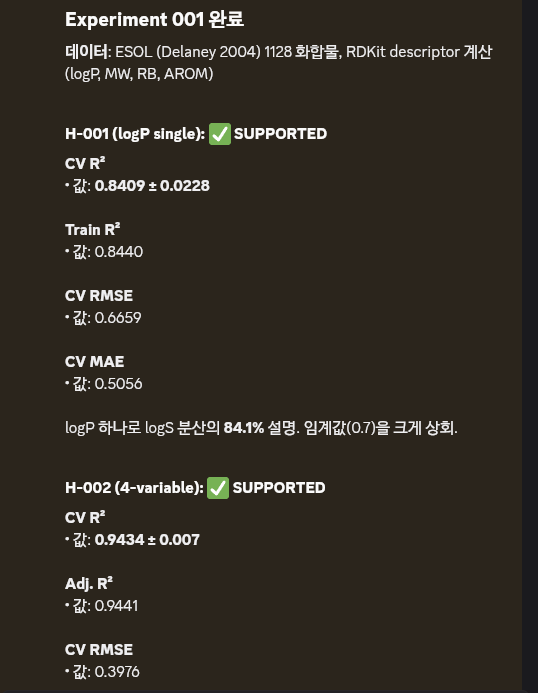
\includegraphics[width=\linewidth]{docs/figures/esol-6-result.png}\par\smallskip{\footnotesize\color{muted} 가설별 결과 (CV R², RMSE 등)}
\end{minipage}\hfill
\begin{minipage}[t]{0.48\linewidth}\vspace{0pt}\centering
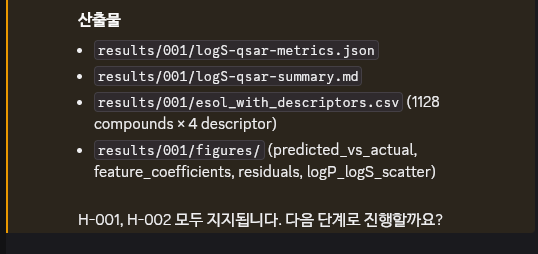
\includegraphics[width=\linewidth]{docs/figures/esol-7-outputs.png}\par\smallskip{\footnotesize\color{muted} 산출물 위치와 다음 단계 질문}
\end{minipage}
\end{center}

\subsection*{⑤ 다음 단계}
\begin{msg}
다음 단계 진행
\end{msg}
PI가 다음 단계(잔차 분석, 다중공선성, 비선형 항 탐색, \cmd{FINDINGS.md} 초안)를 제안하고 다시 승인을 묻습니다. 계속하려면 \cmd{승인}, 여기서 멈추려면 그냥 두면 됩니다.
\begin{center}
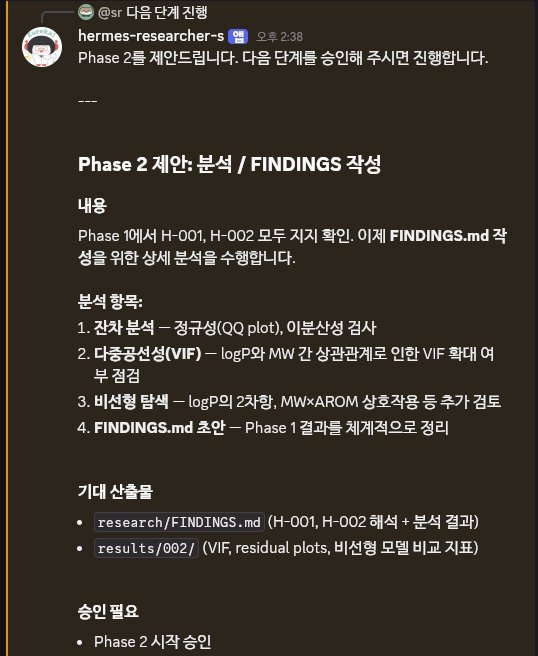
\includegraphics[width=0.55\linewidth]{docs/figures/esol-8-next.png}\par\smallskip
{\footnotesize\color{muted} 다음 단계 제안과 승인 요청}
\end{center}

\tip{이 예시에서 볼 것}{직원은 정의가 애매하면 \textbf{먼저 묻고}, 가설 반영·패키지 추가·다음 단계처럼 방향이 바뀌는 곳에서만 승인을 받습니다. 그 사이의 코드 작성·실행·정리는 알아서 합니다.
진행 중에 \cmd{상태 알려줘}를 보내면 언제든 현재 단계를 표로 받아 볼 수 있습니다.}

% ================================================================
\chapter{매일 쓰는 법}

\section{기본 흐름}

\begin{center}
\begin{tikzpicture}[font=\small,node distance=5mm,
  st/.style={draw=accent!70!black,fill=msgbg,rounded corners=3pt,align=center,inner sep=5pt,minimum height=12mm,text width=24mm}]
  \node[st] (a) {\ch{hermes}에서\\주제 말하기};
  \node[st,right=of a] (b) {PI가 채널·\\폴더·kanban 보드 생성};
  \node[st,right=of b] (c) {Phase 시작\\\textbf{승인}};
  \node[st,right=of c] (d) {직원들이\\kanban 카드로 진행};
  \node[st,right=of d] (e) {Phase 끝에\\PI가 보고};
  \foreach \x/\y in {a/b,b/c,c/d,d/e} \draw[-{Latex},thick,accent] (\x) -- (\y);
  \draw[-{Latex},thick,muted,dashed] (e.south) |- ++(0,-6mm) -| node[pos=0.25,below,font=\footnotesize,color=muted]{다음 Phase} (c.south);
\end{tikzpicture}
\end{center}

내가 하는 일은 대부분 \textbf{주제를 말하고, Phase 시작을 승인하고, 보고를 읽는 것}입니다.
Phase 시작을 승인하면 그 안의 kanban 카드·검토·commit·계획된 실험 실행은 PI가 대신 승인합니다.

\section{상황별 방법}

\begin{center}
\small
\begin{longtable}{L{0.22\linewidth} L{0.7\linewidth}}
\toprule
\head \textbf{하고 싶은 것} & \textbf{방법} \\
\midrule
\endhead
새 연구 주제 시작 & \ch{hermes}에서 PI에게 주제를 말합니다 → 이름·태그 확인 → 30초쯤 뒤 새 채널에서 \textbf{내가 첫 메시지}를 보냅니다 (반응이 없으면 그 채널에서 \cmd{/reset}) \\
진행 상황·오늘 할 일 & PI 봇의 \cmd{/brief} (프로젝트 채널은 그 프로젝트만, \ch{hermes}는 전체), 매일 09:00 자동 브리핑, 또는 \cmd{진행 상황 알려줘} \\
특정 직원에게 직접 & \cmd{@analyst ...}처럼 멘션합니다. PI는 끼어들지 않습니다 \\
내가 승인할 것 & FINDINGS·HYPOTHESES·목표 변경, 다음 Phase 시작, 계획에 없는 실험, 자원 한도 초과, 삭제·되돌리기, 패키지 추가(\cmd{uv add}) \\
보고 받는 때 & Phase가 끝날 때와 막혔을 때만. 중간이 궁금하면 묻거나 \cmd{/brief} \\
막힌 일 & 2번 막히면 차단 감시가 Claude 진단 결과를 \ch{hermes}에 올립니다. ``연구자 결정 필요''에만 답합니다 \\
규칙(SOUL) 고치기 & \cmd{souls/<역할>.md}를 고칩니다 → \cmd{bash install_souls.sh} → 그 채널에서 그 봇에게 \cmd{/reset}. PI 핵심 규칙 \cmd{souls/pi-rules.md}는 고치면 바로 반영됩니다 \\
설정 전체 점검 & \cmd{python3 tools/lab.py check} \\
계산 노드에서 GPU 실험 & \cmd{bash tools/hpc.sh run <프로젝트 폴더> \"<명령>\" -p <파티션> --gres=gpu:1} (\ref{sec:hpc}절) \\
프로젝트 정리 & \cmd{python3 newproject.py remove <이름>}. 채널은 \cmd{archive-<이름>}으로, 폴더는 \cmd{_archive/}로 보관합니다. 미리보기는 \cmd{--dry-run} \\
업데이트 받기 & \cmd{cd ~/Projects/hermes-team && git pull && bash extras/install_extras.sh && bash install_souls.sh} \\
\bottomrule
\end{longtable}
\end{center}

\section{프로젝트 폴더 안내}
\label{sec:projtree}
\does{PI가 새 프로젝트를 만들면 생기는 \cmd{~/Projects/<프로젝트>/} 안의 폴더가 각각 무엇이고, 누가 쓰고, 내가 볼 곳은 어디인지 정리합니다.}

\subsection{왜 이렇게 나눴나: 연구자의 생각 순서를 폴더로}
이 폴더 구조는 연구자가 머릿속에서 하는 일 --- \textbf{질문을 세우고, 가설을 세우고, 실험으로 확인하고, 결과를 해석해 다음 결정을 내리는 순환} --- 을 그대로 파일로 옮긴 것입니다.
순환의 한 단계가 폴더(또는 파일) 하나입니다.

\begin{center}
\begin{tikzpicture}[font=\small,
  st/.style={draw=navy!70,fill=white,rounded corners=4pt,align=center,text width=30mm,minimum height=17mm,inner sep=4pt},
  num/.style={circle,fill=accent,text=white,font=\scriptsize\bfseries,inner sep=1.2pt,minimum size=4.2mm},
  ap/.style={draw=warnc,fill=warnbg,text=warnc,rounded corners=2pt,font=\scriptsize\bfseries,inner sep=1.5pt},
  arr/.style={-{Latex[length=2.4mm]},thick,accent}]
  \node[st] (q) at (0,0)    {\textbf{질문}\\[1pt]{\footnotesize\ttfamily research/OPEN\_QUESTIONS}};
  \node[st] (h) at (38mm,0) {\textbf{가설}\\[1pt]{\footnotesize\ttfamily research/HYPOTHESES}};
  \node[st] (e) at (76mm,0) {\textbf{실험 계획}\\[1pt]{\footnotesize\ttfamily experiments/<ID>.yaml}};
  \node[st] (x) at (114mm,0) {\textbf{실행}\\[1pt]{\footnotesize\ttfamily src/ · hpc.sh}\\[1pt]{\scriptsize\color{muted} coder · analyst}};
  \node[st] (r) at (114mm,-30mm) {\textbf{결과 (측정값)}\\[1pt]{\footnotesize\ttfamily results/<ID>/}\\[1pt]{\scriptsize\color{muted} analyst}};
  \node[st] (f) at (76mm,-30mm) {\textbf{해석 · 발견}\\[1pt]{\footnotesize\ttfamily research/FINDINGS}};
  \node[st] (s) at (38mm,-30mm) {\textbf{상태 · 결정}\\[1pt]{\footnotesize\ttfamily RESEARCH\_STATE}\\{\footnotesize\ttfamily DECISIONS}\\[1pt]{\scriptsize\color{muted} PI}};
  \node[st,draw=muted,dashed,fill=accentlight] (lit) at (0,-30mm) {\textbf{근거 (문헌)}\\[1pt]{\footnotesize\ttfamily docs/literature/}\\[1pt]{\scriptsize\color{muted} scholar}};
  \foreach \n/\k in {q/1,h/2,e/3,x/4,r/5,f/6,s/7} \node[num] at (\n.north west) {\k};
  \draw[arr] (q) -- (h); \draw[arr] (h) -- (e); \draw[arr] (e) -- (x);
  \draw[arr] (x) -- (r); \draw[arr] (r) -- (f); \draw[arr] (f) -- (s);
  \draw[arr] (s.north) -- ++(0,6mm) -| node[pos=0.25,above,font=\scriptsize,text=muted]{다음 질문} ([xshift=8mm]q.south);
  \draw[-{Latex[length=2mm]},thick,muted,dashed] ([xshift=-8mm]lit.north) -- ([xshift=-8mm]q.south);
  \node[ap,anchor=south east] at ([xshift=-2mm]h.north east) {승인};
  \node[ap,anchor=south east] at ([xshift=-2mm]e.north east) {승인};
  \node[ap,anchor=north east] at ([xshift=-2mm]f.south east) {승인};
\end{tikzpicture}
\end{center}

이렇게 나눈 이유는 네 가지입니다.
\begin{itemize}
\item \textbf{AI 직원은 대화가 끝나면 잊습니다.} 새 대화를 열거나 \cmd{/reset}하면 앞의 맥락이 사라집니다.
  그래서 ``지금 어디까지 왔고 무엇을 믿고 있나''를 파일로 남겨, 어느 직원이 언제 이어받아도 같은 출발점에서 시작하게 했습니다.
  \cmd{AGENTS.md}가 작업 전에 \cmd{RESEARCH_STATE}·\cmd{HYPOTHESES}부터 읽게 하는 것도 이 때문입니다.
\item \textbf{측정값과 해석을 나눕니다.} \cmd{results/}에는 숫자만, \cmd{FINDINGS}에는 그 숫자로 무엇을 말할 수 있는지(관찰·해석·한계)를 따로 적습니다.
  AI가 그럴듯한 해석을 사실처럼 쓰는 일을 막고, 나중에 해석만 고쳐 쓸 수 있습니다.
\item \textbf{승인은 연구 방향이 바뀌는 곳에만 둡니다.} 가설을 세우거나 바꿀 때, 실험을 실제로 돌릴 때, 발견을 기록할 때(그림의 \textbf{승인})만 연구자에게 묻고,
  나머지 반복 작업은 직원들이 알아서 합니다. 그래서 내 일은 ``판단''에 집중됩니다.
\item \textbf{같은 실험을 다시 돌릴 수 있게 합니다.} 실험 명세에 실행 명령·코드 버전(commit)·성공 기준을 적고, 결과를 같은 실험 ID 폴더에 모읍니다.
  몇 달 뒤에도 ``어떤 코드로, 어떤 설정으로 나온 숫자인지'' 추적할 수 있습니다.
\end{itemize}

\subsection{폴더별 안내}
새 프로젝트 폴더에는 아래 항목이 생깁니다. 대부분은 직원들이 규칙(\cmd{AGENTS.md})에 따라 채우므로, 내가 직접 고칠 곳은 거의 없습니다.

\begin{center}
\small
\begin{longtable}{L{0.24\linewidth} L{0.42\linewidth} L{0.24\linewidth}}
\toprule
\head \textbf{경로} & \textbf{무엇} & \textbf{누가 쓰나} \\
\midrule
\endhead
\multicolumn{3}{l}{\textbf{규칙과 설정}} \\*
\cmd{AGENTS.md} & 이 프로젝트의 규칙: 이름·태그, 먼저 읽을 파일, 자동 허용/승인 필요/금지, 코드 위임 방법 & PI가 만들 때 작성 \\
\cmd{config/} & \cmd{project.yaml}(목적·실행 환경), \cmd{policy.yaml}(승인 규칙), \cmd{resource_limits.yaml}(GPU·시간 한도) & 처음 그대로. 바꿀 때는 나 \\
\midrule
\multicolumn{3}{l}{\textbf{연구 기록} --- \textbf{내가 가장 자주 읽는 곳}} \\*
\cmd{research/RESEARCH_STATE.md} & 목표, 현재 단계, 다음 행동, 최근 실험, 결정 기록 & PI (승인된 내용 반영) \\
\cmd{research/HYPOTHESES.md} & 가설과 예측·반증 조건 (\cmd{H-001} …) & 수정안은 직원, \textbf{반영은 내 승인 후} \\
\cmd{research/FINDINGS.md} & 확인된 결과: 관찰·해석·한계를 나눠 기록 (\cmd{F-001} …) & analyst 수정안 → \textbf{내 승인 후} \\
\cmd{research/OPEN_QUESTIONS.md} & 아직 풀리지 않은 질문과 우선순위 & 직원 제안 → 내 승인 \\
\cmd{research/DECISIONS.md} & 중요한 설계 결정과 이유 & PI \\
\midrule
\multicolumn{3}{l}{\textbf{실험}} \\*
\cmd{experiments/} & 실험 명세 \cmd{<실험ID>.yaml}: 무엇을, 어떤 명령으로, 성공 기준, 승인 상태. \cmd{templates/}는 빈 양식 & analyst 작성, \textbf{실행은 내 승인 후} \\
\cmd{schemas/} & 실험 명세가 지켜야 할 형식(JSON Schema) & 처음 그대로 \\
\cmd{results/<실험ID>/} & 실험 결과: \cmd{summary.md}, \cmd{metrics.json}, 그림(\cmd{figures/}) & analyst \\
\cmd{plots/} & 결과 그림을 그리는 코드 (\cmd{plot_<실험ID>.py}). \cmd{results/}만 읽음 & analyst가 Claude Code에 맡김 \\
\midrule
\multicolumn{3}{l}{\textbf{코드와 Python 환경}} \\*
\cmd{src/} & 실험 코드 (필요해지면 생깁니다) & coder가 Claude Code에 맡김 \\
\cmd{scripts/researchctl} & 점검 도구: \cmd{doctor}(환경 점검·수리), \cmd{list}·\cmd{validate}(명세 확인) & 직원이 실행 \\
\cmd{pyproject.toml}, \cmd{uv.lock} & 이 프로젝트의 Python 패키지 목록과 정확한 버전 & \cmd{uv add} (패키지 추가는 \textbf{내 승인}) \\
\cmd{.venv/} (숨김) & 실제 설치된 환경. git에 올리지 않음 & \cmd{uv}가 자동 \\
\midrule
\multicolumn{3}{l}{\textbf{문서}} \\*
\cmd{docs/literature/} & 문헌 조사 보고서, \cmd{references.bib}, 내가 구한 PDF(\cmd{pdfs/}) & scholar. \textbf{PDF는 내가 넣어도 됨} \\
\cmd{docs/paper/} & 논문 초안 (필요해지면 생깁니다) & writer가 Claude Code에 맡김 \\
\cmd{docs/*_ko.md} & 이 템플릿의 설계 설명서 (구조, 운영, 보안, 용어) & 읽기용 \\
\midrule
\multicolumn{3}{l}{\textbf{예시와 참고 (처음에는 건드리지 않음)}} \\*
\cmd{deployment/} & Slurm·systemd·cron 예시 파일 & 참고용. GPU 실행은 \ref{sec:hpc}절 \cmd{hpc.sh} \\
\cmd{monitoring/} & 실험 기록·관측 안내 & 참고용 \\
\cmd{skills/} & 반복 작업 절차(스킬) 양식, 예: 결과 분석 절차 & 직원이 참고 \\
\cmd{README_ko.md} & 이 템플릿 자체의 소개 (예시 프로젝트 이름이 섞여 있음) & 참고용 \\
\bottomrule
\end{longtable}
\end{center}

\tip{매일 볼 곳은 세 군데}{① \cmd{research/RESEARCH_STATE.md} --- 지금 어디까지 왔고 다음에 뭘 하는지.
② \cmd{research/FINDINGS.md} --- 지금까지 확인된 결과.
③ \cmd{results/<실험ID>/summary.md} --- 방금 끝난 실험 하나의 요약.
나머지는 PI의 보고나 \cmd{/brief}로 충분합니다.}

\info{승인이 필요한 곳은 정해져 있습니다}{\cmd{research/}의 가설·결과 수정, 실험 실행(명세의 \cmd{approval}), 패키지 추가(\cmd{uv add}), 파일 삭제는 직원이 먼저 Discord에서 묻습니다.
자세한 목록은 그 프로젝트의 \cmd{AGENTS.md} ``권한 규칙''과 \cmd{config/policy.yaml}에 있습니다.}

\section{계산 노드에서 실험 돌리기 (hpc.sh)}
\label{sec:hpc}
\does{GPU 실험을 Slurm으로 계산 노드(예: gnode5)에 보내고, 결과를 gnode1의 \cmd{/data}로 받아 옵니다.}

gnode1의 \cmd{/ai}와 \cmd{/data}는 다른 노드에서 보이지 않습니다. 그래서 \cmd{~/Projects}에서 \cmd{sbatch}를 바로 하면 계산 노드가 로그 파일을 열지 못해 job이 시작도 못 하고 끝납니다(\cmd{RaisedSignal:53}).
또 계산 노드는 인터넷이 안 되어 거기서 패키지를 설치할 수 없습니다. \cmd{tools/hpc.sh}가 이 일을 대신합니다.

\begin{center}
\small
\begin{tabular}{L{0.05\linewidth} L{0.85\linewidth}}
\toprule
\head & \textbf{\cmd{hpc.sh run}이 하는 일} \\
\midrule
1 & gnode1에서 \cmd{uv}로 Python과 패키지를 설치해 묶음 하나로 \cmd{/home/<계정>/hpc/envs/}에 둡니다. 패키지가 바뀔 때만 다시 만듭니다 \\
2 & 프로젝트 폴더를 \cmd{/home/<계정>/hpc/in/}에 복사하고 \cmd{sbatch}로 제출합니다 \\
3 & 계산 노드가 코드와 환경을 자기 로컬 디스크(\cmd{/var/tmp/<계정>})에 풀어 계산합니다. 환경은 노드마다 처음 한 번만 풉니다 \\
4 & 끝나면(실패해도) \cmd{out/} 폴더와 종료 코드만 \cmd{/home}으로 돌려놓고 로컬 작업 폴더를 지웁니다 \\
5 & gnode1이 결과를 \cmd{/data/<계정>/results/}로 옮기고 \cmd{/home}에 올렸던 것을 지웁니다 \\
\bottomrule
\end{tabular}
\end{center}

\begin{center}
\begin{tikzpicture}[font=\small,
  zone/.style={draw=navy!60,rounded corners=6pt,fill=#1,inner sep=6pt},
  box/.style={draw=navy!70,fill=white,rounded corners=3pt,align=center,text width=34mm,minimum height=10mm,inner sep=3pt,font=\footnotesize},
  num/.style={circle,fill=accent,text=white,font=\scriptsize\bfseries,inner sep=1pt,minimum size=4.2mm},
  arr/.style={-{Latex[length=2.2mm]},thick,accent},
  ttl/.style={font=\small\bfseries,text=navy}]
  % gnode1
  \node[box] (proj) at (0,-17mm)  {\textbf{내 프로젝트}\\{\ttfamily \textasciitilde/Projects/<이름>}};
  \node[box] (envb) at (0,0)      {\textbf{환경 만들기}\\{\ttfamily uv sync → tar}};
  \node[box] (res)  at (0,-34mm)  {\textbf{결과 도착}\\{\ttfamily /data/<계정>/results/}};
  % /home (NFS)
  \node[box] (envs) at (50mm,0)      {{\ttfamily hpc/envs/}\\환경 묶음 (재사용)};
  \node[box] (in)   at (50mm,-17mm)  {{\ttfamily hpc/in/}\\코드 복사본};
  \node[box] (out)  at (50mm,-34mm)  {{\ttfamily hpc/out/}\\\texttt{out/}·로그·종료 코드};
  % compute node
  \node[box] (nenv) at (100mm,0)     {\textbf{환경 풀기}\\{\ttfamily /var/tmp/<계정>/env}\\(노드마다 처음 한 번)};
  \node[box] (run)  at (100mm,-17mm) {\textbf{계산}\\{\ttfamily /var/tmp/<계정>/job/<번호>}};
  \node[box] (nout) at (100mm,-34mm) {\textbf{\texttt{out/}만 돌려보냄}\\작업 폴더는 지움};
  \begin{scope}[on background layer]
    \node[zone=accentlight,fit=(proj)(envb)(res),label={[ttl]above:gnode1 (로그인·Hermes)}] {};
    \node[zone=msgbg,fit=(envs)(in)(out),label={[ttl]above:/home/<계정> (NFS, 거쳐 가는 곳)}] {};
    \node[zone=codebg!8,fit=(nenv)(run)(nout),label={[ttl]above:계산 노드 (예: gnode5)}] {};
  \end{scope}
  \draw[arr] (proj) -- (envb);
  \draw[arr] (envb.east) -- node[num,above=1pt,pos=0.5]{1} (envs.west);
  \draw[arr] (proj.east) -- node[num,above=1pt,pos=0.5]{2} (in.west);
  \draw[arr] (envs) -- node[num,above=1pt]{3} (nenv);
  \draw[arr] (in) -- node[num,above=1pt]{3} (run);
  \draw[arr] (nenv) -- (run);
  \draw[arr] (run) -- (nout);
  \draw[arr] (nout) -- node[num,above=1pt]{4} (out);
  \draw[arr] (out) -- node[num,above=1pt]{5} (res);
  \node[font=\scriptsize,text=muted,anchor=north,align=center] at (50mm,-44mm) {끝나면 \texttt{in/}·\texttt{out/}은 비워집니다. 환경 묶음만 남아 다음에 다시 씁니다.};
\end{tikzpicture}
\end{center}

\subsection{처음 한 번}
결과가 거쳐 가는 곳(\cmd{/home})과 도착하는 곳(\cmd{/data})을 만들고, 쓸 \textbf{파티션 이름}을 확인합니다.
\begin{sh}
mkdir -p /home/$USER/hpc /data/$USER/results && echo OK
sinfo -s
\end{sh}
\ok{\cmd{OK}가 나오고, \cmd{sinfo -s}의 \cmd{PARTITION} 칸에 파티션 이름(예: \cmd{p6k1})이 보입니다.}
\info{파티션과 노드는 다릅니다}{\cmd{gnode5} 같은 것은 \textbf{노드}(컴퓨터) 이름이고, \cmd{-p}에는 노드 묶음인 \textbf{파티션} 이름을 씁니다. \cmd{-p gnode5}라고 쓰면 \cmd{invalid partition}으로 거절됩니다.
어떤 노드가 어느 파티션에 있고 GPU가 몇 장인지는 \cmd{sinfo -N -n gnode5 -O NodeList,Partition,Gres}로 봅니다. 특정 노드에서 돌리고 싶으면 \cmd{-w gnode5}를 더합니다.}
\warn{\cmd{mkdir: Permission denied}가 나오면}{\cmd{/data/<계정>} 폴더가 없고 만들 권한도 없는 것입니다. 관리자에게 gnode1의 \cmd{/data/<계정>}을 만들어 달라고 부탁합니다.
다른 곳에 결과를 받으려면 \cmd{echo 'export HPC_RESULTS=<쓸 수 있는 폴더>/results' >> ~/.bashrc} 후 \cmd{source ~/.bashrc}.}

\subsection{시험해 보기}
패키지 없는 작은 프로젝트로 한 번 돌려 봅니다. 계산 노드 이름과 GPU가 보이면 준비가 끝난 것입니다.
\begin{sh}
mkdir -p ~/Projects/hpctest && cd ~/Projects/hpctest && uv init -q --bare
cat > hello.py <<'END'
import os, socket, platform
os.makedirs("out", exist_ok=True)
with open("out/hello.txt", "w") as f:
    f.write(f"host={socket.gethostname()}\npython={platform.python_version()}\ncwd={os.getcwd()}\n")
END
bash ~/Projects/hermes-team/tools/hpc.sh run ~/Projects/hpctest \
  'python hello.py; nvidia-smi > out/gpu.txt; echo "CUDA_VISIBLE_DEVICES=$CUDA_VISIBLE_DEVICES" >> out/hello.txt' \
  -p <파티션> --gres=gpu:1 -t 00:05:00
cat /data/$USER/results/hpctest-*/hello.txt
\end{sh}
\begin{out}
host=gnode5
python=3.15.2
cwd=/var/tmp/minji/job/999
CUDA_VISIBLE_DEVICES=0
\end{out}
\ok{\cmd{host}가 gnode1이 아닌 계산 노드이고, \cmd{cwd}가 계산 노드의 로컬 디스크(\cmd{/var/tmp})이며, \cmd{CUDA_VISIBLE_DEVICES}에 숫자 하나가 있습니다.
\cmd{gpu.txt}에 GPU 표가 있습니다.}
\tip{\cmd{nvidia-smi}에 GPU가 여러 장 보여도 괜찮습니다}{노드의 GPU가 모두 보일 수 있지만, 내 job이 쓸 GPU는 \cmd{CUDA_VISIBLE_DEVICES}가 정합니다. PyTorch 등은 이 값을 따르므로 \cmd{--gres=gpu:1}이면 1장만 씁니다.}

\subsection{실행}
실행 명령은 따옴표로 묶고, 뒤에는 평소 \cmd{sbatch}에 주던 옵션을 그대로 씁니다.
\begin{sh}
bash ~/Projects/hermes-team/tools/hpc.sh run ~/Projects/<프로젝트> "python train.py" \
  -p <파티션> --gres=gpu:1 -t 01:00:00
\end{sh}
\begin{out}
[hpc] 환경 만들기: /var/tmp/minji/env/<프로젝트>-3f9a1c2b7d4e
[hpc] 코드 올리기: /home/minji/hpc/in/<프로젝트>-1105-142233-5120
[hpc] 제출: job 931 (<프로젝트>-1105-142233-5120)
job 931 → /data/minji/results/<프로젝트>-1105-142233-5120-931  (exit 0)
\end{out}
\ok{마지막 줄이 \cmd{(exit 0)}입니다. 결과 폴더에 \cmd{out/}에 쓴 파일, 화면 출력 \cmd{run.log}, Slurm 로그 \cmd{slurm.log}, \cmd{exit_code}가 있습니다.}

\begin{center}
\small
\begin{tabular}{L{0.38\linewidth} L{0.52\linewidth}}
\toprule
\head \textbf{명령} & \textbf{하는 일} \\
\midrule
\cmd{hpc.sh run <폴더> "<명령>" [옵션]} & 제출하고 끝날 때까지 기다렸다가 결과를 가져옵니다 \\
\cmd{hpc.sh submit <폴더> "<명령>" [옵션]} & 제출만 합니다. 긴 실험은 이것으로 \\
\cmd{hpc.sh status} & 돌고 있는 job과 아직 안 가져온 결과 \\
\cmd{hpc.sh fetch <job번호|all>} & 끝난 job의 결과를 가져옵니다 \\
\bottomrule
\end{tabular}
\end{center}

\warn{규칙 두 가지}{① 프로그램은 결과를 \textbf{\cmd{out/} 폴더에} 써야 돌아옵니다. 다른 곳에 쓴 파일은 job이 끝나면 지워집니다.
\cmd{results/}처럼 다른 폴더에 쓰는 코드라면 명령 끝에 복사를 붙입니다. 예: \cmd{"python src/logS_qsar.py && cp -r results out/"} (\ref{sec:esol}절 실험을 계산 노드에서 다시 돌린 명령).\par
② 데이터셋은 계산 노드에서 보이지 않습니다. 필요한 데이터는 프로젝트 폴더 안에 두거나, 관리자와 정한 방법으로 옮깁니다.}

\tip{실패했을 때}{\cmd{exit} 숫자가 0이 아니면 결과 폴더의 \cmd{run.log}(프로그램 오류)와 \cmd{slurm.log}(노드·환경 문제)를 봅니다.
\cmd{exit 90}은 계산 노드 로컬 디스크가 20GB보다 적게 남아 시작하지 않은 것입니다.}

\info{걸리는 시간}{패키지를 바꾼 뒤 첫 실행만 환경을 다시 묶느라 몇 분 걸립니다(torch를 넣은 환경에서 약 5분). 패키지가 그대로면 환경을 다시 만들지도 풀지도 않아서 제출부터 결과까지 몇 초입니다(같은 환경 두 번째 실행 3초).
그래서 패키지를 이것저것 바꿔 보는 동안은 gnode1에서 \cmd{uv add}와 \cmd{uv run}으로 시험하고, 패키지가 정해진 뒤 계산 노드로 보냅니다.}

\section{새 직원 추가하기}
\label{sec:newmember}
\does{6명 말고 직원을 더 둡니다. 예: 통계 검토만 맡는 \cmd{stats}.}

설치 때 한 일을 \textbf{그 직원 한 명에게만} 다시 하는 것입니다. 아래에서 \cmd{stats}를 새 이름으로 바꿔 읽습니다.
이름은 영어 소문자로 짓습니다.

\begin{enumerate}
\item \textbf{Discord 봇 만들기.} 4.1절을 그대로 한 번 더 합니다. Application ID, 토큰, 봇 ID를 기록표 빈 줄에 적습니다.
\item \textbf{profile 만들고 토큰 넣기.} 4.3절처럼 PI를 복제한 뒤 자기 봇 토큰을 넣습니다.
\begin{sh}
hermes profile create stats --clone --description "통계 검토 담당. \
분석 결과의 검정 방법과 수치를 확인해 보고한다. 직접 수정하지 않는다."
hermes -p stats gateway setup        # Discord → stats 봇 토큰 → y → Enter
hermes -p stats chat -q "OK라고만 답해"
\end{sh}
\item \textbf{모델 확인.} PI를 복제했으므로 모델 설정도 PI와 같습니다. 주 모델은 로컬 모델이고, 예비 모델은 Claude입니다. 두 줄로 확인합니다.
\begin{sh}
hermes -p stats config get model.default     # qwen3.6-35b-a3b
hermes -p stats fallback list                # 1. claude-opus-5-5
\end{sh}
ChatGPT를 주 모델로 쓰려면 \ref{sec:togpt}절의 로그인 한 줄과 모델 두 줄을 \cmd{-p stats}로 실행합니다.
\item \textbf{역할(SOUL) 쓰기.} 비슷한 직원의 파일을 복사해 고칩니다. PI가 일을 맡기려면 PI도 이 직원을 알아야 합니다.
\begin{sh}
cd ~/Projects/hermes-team
cp souls/reviewer.md souls/stats.md
nano souls/stats.md          # 이름·담당·할 일·하지 않을 일을 고칩니다
nano souls/pi.md             # 맨 위 직원 표에 stats 줄을 하나 추가합니다
nano souls/_team_ids.md      # "- scholar: ..." 아래에 - stats: `<@봇ID>` 줄 추가
\end{sh}
\item \textbf{팀 설정에 넣기.} \cmd{team.json}의 \cmd{"profiles"} 목록 끝에 \cmd{"stats"}를 더합니다. 앞 항목 뒤에 쉼표를 잊지 않습니다.
생각 깊이를 정하려면 \cmd{"reasoning"}에도 \cmd{"stats": "medium"}을 더합니다.
\begin{filebox}{team.json (바뀐 부분)}
\begin{code}
  "profiles": ["default", "coder", "analyst", "reviewer", "writer", "scholar", "stats"],
\end{code}
\end{filebox}
\item \textbf{적용.} 6.2절 네 줄을 그대로 다시 실행합니다. 이번엔 새 직원까지 포함됩니다.
\begin{sh}
python3 tools/lab.py env
python3 tools/lab.py reasoning
python3 newproject.py sync
bash install_souls.sh
\end{sh}
\item \textbf{슬래시 명령 등록.} 6.3절을 \cmd{stats} 한 명에게만 합니다.
\begin{sh}
echo 'DISCORD_COMMAND_SYNC_POLICY=bulk' >> ~/.hermes/profiles/stats/.env
hermes gateway restart --all
sleep 30
sed -i '/^DISCORD_COMMAND_SYNC_POLICY=bulk$/d' ~/.hermes/profiles/stats/.env
hermes gateway restart --all
\end{sh}
\end{enumerate}
\ok{\cmd{python3 tools/lab.py check}에 \cmd{stats}가 나오고 문제가 없습니다. 프로젝트 채널에서 \cmd{@stats 넌 누구야?}에 새 역할로 답합니다.}
\info{원래 있던 직원은 건드리지 않습니다}{위 단계는 모두 새 직원 한 명에게만 하거나, 6명에게 다시 해도 결과가 같은 명령입니다. 기존 직원의 설정과 기억은 그대로입니다.}

% ================================================================
\chapter{문제 해결}

\section{먼저 해 볼 것}
\begin{sh}
python3 ~/Projects/hermes-team/tools/lab.py check     # 무엇이 틀렸는지 + 고치는 명령
hermes gateway status                                 # 게이트웨이가 도는지
hermes doctor                                         # Hermes 자체 진단
\end{sh}
로그 위치: PI는 \cmd{~/.hermes/logs/}, 직원은 \cmd{~/.hermes/profiles/<이름>/logs/}.

\section{증상별 해결}

\begin{center}
\small
\begin{longtable}{L{0.32\linewidth} L{0.6\linewidth}}
\toprule
\head \textbf{증상} & \textbf{원인 / 해결} \\
\midrule
\endhead
\multicolumn{2}{l}{\color{accent}\bfseries 설치} \\
\cmd{hermes: command not found} & \cmd{source ~/.bashrc} 또는 터미널을 새로 엽니다 \\
\cmd{install_souls.sh}가 ``채우지 않은 ID'' & 6.1절 \cmd{team.json}, \cmd{_team_ids.md}의 빈 자리를 채웁니다 \\
\cmd{git switch main} 실패 & 저장소 기본 브랜치가 \cmd{master}입니다. 2.1절 \cmd{init.defaultBranch main}을 해 두면 새 저장소는 \cmd{main}이 됩니다 \\
\midrule
\multicolumn{2}{l}{\color{accent}\bfseries Discord 봇} \\
자동완성에 봇이 안 보임 & 서버에 초대되지 않았습니다 → 4.1절 4번을 \textbf{그 봇의} Application ID로 다시 \\
멘션했는데 반응이 없음 & 역할(role)을 골랐습니다 → \textbf{APP} 표시 항목을 고르거나 \cmd{<@봇ID>}를 직접 입력 \\
봇이 오프라인 / 하나를 켜면 다른 게 꺼짐 & 토큰 중복입니다 (\cmd{--clone}이 PI 토큰을 복사) → \cmd{lab.py check}로 확인 → 4.3.2절 다시 \\
봇이 접속하지 못함 & Message Content Intent가 꺼져 있습니다 → 4.1절 3번 \\
PI가 멘션해도 직원이 무시함 & 협업 설정 → \cmd{python3 tools/lab.py env} 후 \cmd{hermes gateway restart --all} \\
다른 직원만 멘션했는데 PI도 길게 답함 & 정상은 \cmd{—} 한 글자입니다. PI SOUL이 옛것 → \cmd{install_souls.sh} + \cmd{/reset} \\
새 프로젝트 만들 때 HTTP 403 & 6.4절 카테고리 권한, \cmd{team.json}의 \cmd{category_id} 확인 \\
\midrule
\multicolumn{2}{l}{\color{accent}\bfseries 모델} \\
답은 오는데 \cmd{/slots}의 \cmd{id_task}가 그대로 & 로컬 모델이 꺼져 Claude 예비가 답하는 중입니다 → \ref{sec:modelcheck}절. 오래 두면 Claude 사용량이 빨리 찹니다 \\
\cmd{429} / rate limit & ChatGPT 사용 한도입니다. kanban 카드는 대기했다가 자동으로 다시 시작됩니다. 기다리면 됩니다 \\
\midrule
\multicolumn{2}{l}{\color{accent}\bfseries 동작} \\
규칙을 바꿨는데 예전처럼 행동함 & 열린 대화는 예전 SOUL을 가지고 있습니다 → 그 채널에서 그 봇에게 \cmd{/reset} \\
\cmd{config.yaml}을 고쳤는데 그대로 & \texttt{\# discord:}로 시작하는 주석 예시를 고친 것입니다. discord 설정은 \cmd{newproject.py sync}가 관리합니다 \\
kanban 카드 결과 파일이 사라짐 & 작업 위치가 \cmd{scratch}였습니다 → 항상 \cmd{dir:<프로젝트 경로>} (PI SOUL에 규칙 있음) \\
kanban 카드가 \cmd{blocked} & 같은 원인으로 2번 실패했습니다. 원인을 고친 뒤 \cmd{hermes kanban --board <p> unblock <id>} \\
브리핑 로그에 \cmd{BLOCKED: script execution via -e/-c} & 무인 실행에서 \cmd{python -c} 같은 명령이 막힌 것입니다. 다른 방법으로 다시 시도하므로 무시해도 됩니다 \\
\cmd{uv} 없음 / \cmd{.venv} 깨짐 & 그 프로젝트 폴더에서 \cmd{bash scripts/researchctl doctor --fix} \\
\bottomrule
\end{longtable}
\end{center}

% ================================================================
\appendix
\renewcommand{\thechapter}{\Alph{chapter}}

\chapter{지금 연구실을 다른 컴퓨터로 옮기기}
\label{app:move}

같은 봇과 같은 프로젝트를 그대로 쓰는 경우입니다. 새로 만들지 않으므로 3\textasciitilde6장 대부분이 필요 없습니다.

\begin{enumerate}[label=\textbf{\arabic*.}]
\item \textbf{새 컴퓨터}에서 2.1\textasciitilde2.5절을 합니다 (도구 설치, Claude·Antigravity 로그인). 로컬 모델 서버도 새 컴퓨터에서 돌고 있어야 합니다.
\item \textbf{원래 컴퓨터}에서 백업합니다. 끝날 때 나오는 \textbf{빠진 파일 보고}를 확인합니다.
\begin{sh}
hermes backup                         # ~/hermes-backup-<시각>.zip (설정, 토큰, 기억, profile 전부)
tar czf ~/projects.tgz -C ~ Projects  # hermes-team + 모든 연구 프로젝트
\end{sh}
\item \textbf{원래 컴퓨터의 게이트웨이를 멈춥니다.} 같은 토큰으로 두 곳이 동시에 접속하면 안 됩니다.
\item 두 파일을 새 컴퓨터로 복사한 뒤 복원합니다.
\begin{sh}
hermes import ~/hermes-backup-<시각>.zip
tar xzf ~/projects.tgz -C ~
\end{sh}
\item \textbf{사용자 이름(홈 경로)이 바뀌었다면} 프로젝트 경로를 고치고 채널 연결을 다시 만듭니다.
\begin{sh}
cd ~/Projects/hermes-team
sed -i "s#/home/<예전사용자>/#$HOME/#g" projects.json
python3 newproject.py sync
\end{sh}
\item 로컬 모델 포트가 바뀌었다면 \ref{sec:changemain}절 ``로컬 모델 포트가 바뀌었을 때'' 명령으로 4명의 주소를 고칩니다.
\item 권한과 자동 장치를 설치합니다.
\begin{sh}
python3 tools/lab.py agy-perms
bash extras/install_extras.sh
bash install_souls.sh
python3 tools/lab.py check
\end{sh}
\item 6.8절(재부팅 대비)을 하고 7.2절 시험을 합니다.
\end{enumerate}

\warn{백업 파일은 옮긴 뒤 지웁니다}{\cmd{hermes backup} zip에는 \textbf{봇 토큰과 로그인 정보}가 들어 있습니다.}

\chapter{다른 사람에게 넘기기 (넘겨주는 쪽)}

\cmd{hermes-team} 폴더 자체가 GitHub 저장소입니다. 저장소는 두 개로 나눠 씁니다.
\begin{itemize}
\item \textbf{개발용} \cmd{hermes-team} (비공개): 평소에 고치고 push하는 곳. commit 기록이 모두 남습니다.
\item \textbf{배포용} \cmd{hermes-team-public} (공개): 남에게 주는 곳. commit 기록 없이 \textbf{최신 1개}만 있습니다.
\end{itemize}
배포용을 최신으로 바꿀 때는 개발용에서 commit한 뒤 아래 한 줄을 실행합니다. \cmd{main}에 commit된 파일만 보내고, 보내기 전에 개인 정보를 검사해 섞여 있으면 멈춥니다.
\begin{sh}
bash ~/Projects/hermes-team/tools/publish.sh
\end{sh}
받는 사람에게는 배포용 주소와 이 문서를 주면 2장부터 따라 합니다 (\cmd{git clone https://github.com/<계정>/hermes-team-public.git ~/Projects/hermes-team}).

\begin{itemize}
\item \textbf{저장소에 올라가는 것}: SOUL·템플릿 원본(연구자 이름은 \cmd{{{연구자}}}), 스크립트, 플러그인, 문서
\item \textbf{올라가지 않는 것}: \cmd{team.json}, \cmd{souls/_team_ids.md}, \cmd{projects.json}, \cmd{memories/}, \cmd{state/}, \cmd{logs/}, 슬라이드
\item commit할 때 \cmd{tools/git-hooks/pre-commit}이 연구자 이름·Discord ID·홈 경로·위 파일을 검사해서 섞이면 막습니다.
\item 인터넷 없이 파일로 넘겨야 할 때만 \cmd{bash tools/make_handover.sh}로 \cmd{~/Projects/hermes-team-share.tar}를 만듭니다.
\end{itemize}

\tip{내 연구실을 다시 설치할 때}{직원들이 쌓은 장기 기억은 다시 설치하기 전에 \cmd{bash tools/memories.sh export}로 받아 두고,
설치 후 \cmd{bash tools/memories.sh import} → \cmd{bash install_souls.sh}로 되돌립니다. 새 연구실이면 필요 없습니다.}

\chapter{명령어와 파일 요약}

\section{자주 쓰는 명령}
\begin{center}
\small
\begin{tabular}{L{0.48\linewidth} L{0.44\linewidth}}
\toprule
\head \textbf{명령} & \textbf{뜻} \\
\midrule
\cmd{python3 tools/lab.py check} & 전체 점검 (아무것도 바꾸지 않음) \\
\cmd{hermes gateway status} & 게이트웨이 상태 \\
\cmd{hermes gateway restart --all} & 6명 모두 다시 켜기 \\
\cmd{hermes -p <직원> chat -q "..."} & 터미널에서 직원 한 명에게 한 번 묻기 \\
\cmd{hermes profile list} & 직원(profile) 목록 \\
\cmd{hermes kanban --board <프로젝트> list} & 프로젝트의 kanban 카드 목록 \\
\cmd{hermes cron status} & 아침 브리핑 등 예약 작업 \\
\cmd{python3 newproject.py list} & 등록된 프로젝트·채널 \\
\cmd{python3 newproject.py sync} & 채널 연결 다시 만들기 \\
\cmd{bash install_souls.sh} & 규칙(SOUL) 설치 + 재시작 \\
\cmd{bash extras/install_extras.sh} & 자동 장치 설치 \\
\cmd{bash set_name.sh <이름>} & 연구자 이름 바꾸기 \\
\bottomrule
\end{tabular}
\end{center}

\section{파일 지도}
\begin{filebox}{어디에 무엇이 있나}
\begin{code}
~/Projects/hermes-team/          ← 연구실 "설계도" (이 폴더만 옮기면 같은 연구실을 만들 수 있다)
├── INSTALL.md / INSTALL.tex     이 문서
├── LOCAL_MODEL.md               로컬 모델 설치
├── team.json                    Discord ID, 직원 목록, 생각 깊이 (내 PC 전용)
├── projects.json                프로젝트 ↔ 채널 (newproject.py가 관리, 내 PC 전용)
├── newproject.py                새 프로젝트: 폴더+git+uv, 채널, 채널 연결, kanban 보드
├── install_souls.sh             souls/*.md → 6명의 SOUL.md, 재시작
├── set_name.sh                  연구자 이름 정하기
├── souls/                       직원별 역할·규칙 원본 + _team_ids.md (ID)
├── template/                    새 프로젝트 뼈대
├── tools/lab.py                 설치 도우미: env / reasoning / agy-perms / rename / check
├── tools/hpc.sh                 계산 노드 실행: run / submit / status / fetch (hpc_job.sh와 한 쌍)
├── extras/                      자동 장치 원본 (install_extras.sh가 설치)
└── memories/ state/ logs/       직원 기억 사본, 실행 상태, 기록 (내 PC 전용)

~/.hermes/                       ← Hermes 데이터 (비밀 포함, git에 올리지 않는다)
├── config.yaml  .env  SOUL.md   PI(default)
└── profiles/<직원>/             직원별 config.yaml, .env(봇 토큰), SOUL.md, logs/

~/Projects/<프로젝트>/           ← 연구 프로젝트 하나 (git 저장소)
├── AGENTS.md                    이 프로젝트에서 직원들이 따를 규칙
├── research/                    RESEARCH_STATE, HYPOTHESES, FINDINGS (승인 후에만 수정)
└── experiments/ results/ src/ docs/ scripts/researchctl

/data/<계정>/results/    ← hpc.sh로 계산 노드에서 돌린 실험 결과
/home/<계정>/hpc/                ← hpc.sh가 계산 노드와 주고받는 임시 칸 (공유 디스크, 비워 둔다)
\end{code}
\end{filebox}

\end{document}
